
\documentclass[twoside]{article}
\usepackage{algorithm}
\usepackage{algorithmic}
\usepackage{amssymb,amsmath,amsthm}
\usepackage{graphicx}
\usepackage{preamble}
\usepackage{natbib}
%%%% REMEMBER ME!
%\usepackage[draft]{hyperref}
\usepackage{hyperref}
\usepackage{color}
\usepackage{wasysym}
\usepackage{subfigure}
\usepackage{tabularx}
\usepackage{booktabs}
\usepackage{bm}
\newcommand{\theHalgorithm}{\arabic{algorithm}}
\definecolor{mydarkblue}{rgb}{0,0.08,0.45}
\hypersetup{ %
    pdftitle={},
    pdfauthor={},
    pdfsubject={},
    pdfkeywords={},
    pdfborder=0 0 0,
    pdfpagemode=UseNone,
    colorlinks=true,
    linkcolor=mydarkblue,
    citecolor=mydarkblue,
    filecolor=mydarkblue,
    urlcolor=mydarkblue,
    pdfview=FitH}

\newcolumntype{x}[1]{>{\centering\arraybackslash\hspace{0pt}}m{#1}}
\newcommand{\tabbox}[1]{#1}

\setlength{\marginparwidth}{0.6in}
%%%%%%%%%%%%%%%%%%%%%%%%%%%%%%%%%%%%%%%%%%%%%%%%%%%%%%%%%%
%%%% EDITING HELPER FUNCTIONS  %%%%%%%%%%%%%%%%%%%%%%%%%%%
%%%%%%%%%%%%%%%%%%%%%%%%%%%%%%%%%%%%%%%%%%%%%%%%%%%%%%%%%%

%% NA: needs attention (rough writing whose correctness needs to be verified)
%% TBD: instructions for how to fix a gap ("Describe the propagation by ...")
%% PROBLEM: bug or missing crucial bit 

%% use \fXXX versions of these macros to put additional explanation into a footnote.  
%% The idea is that we don't want to interrupt the flow of the paper or make it 
%% impossible to read because there are a bunch of comments.

%% NA's (and TBDs, those less crucially) should be written so 
%% that they flow with the text.

\definecolor{WowColor}{rgb}{.75,0,.75}
\definecolor{SubtleColor}{rgb}{0,0,.50}

% inline
\newcommand{\NA}[1]{\textcolor{SubtleColor}{ {\tiny \bf ($\star$)} #1}}
\newcommand{\LATER}[1]{\textcolor{SubtleColor}{ {\tiny \bf ($\dagger$)} #1}}
\newcommand{\TBD}[1]{\textcolor{SubtleColor}{ {\tiny \bf (!)} #1}}
\newcommand{\PROBLEM}[1]{\textcolor{WowColor}{ {\bf (!!)} {\bf #1}}}

% as margin notes

\newcounter{margincounter}
\newcommand{\displaycounter}{{\arabic{margincounter}}}
\newcommand{\incdisplaycounter}{{\stepcounter{margincounter}\arabic{margincounter}}}

\newcommand{\fTBD}[1]{\textcolor{SubtleColor}{$\,^{(\incdisplaycounter)}$}\marginpar{\tiny\textcolor{SubtleColor}{ {\tiny $(\displaycounter)$} #1}}}

\newcommand{\fPROBLEM}[1]{\textcolor{WowColor}{$\,^{((\incdisplaycounter))}$}\marginpar{\tiny\textcolor{WowColor}{ {\bf $\mathbf{((\displaycounter))}$} {\bf #1}}}}

\newcommand{\fLATER}[1]{\textcolor{SubtleColor}{$\,^{(\incdisplaycounter\dagger)}$}\marginpar{\tiny\textcolor{SubtleColor}{ {\tiny $(\displaycounter\dagger)$} #1}}}


\newif\ifarXiv
%\arXivtrue

\ifarXiv
	\usepackage[arxiv]{format/icml2013}
\else
	\usepackage[accepted]{format/icml2013}
\fi
%\usepackage[left=1.00in,right=1.00in,bottom=0.25in,top=0.25in]{geometry} %In case we want larger margins for commenting purposes

%% For submission, make all render blank.
%\renewcommand{\LATER}[1]{}
%\renewcommand{\fLATER}[1]{}
%\renewcommand{\TBD}[1]{}
%\renewcommand{\fTBD}[1]{}
%\renewcommand{\PROBLEM}[1]{}
%\renewcommand{\fPROBLEM}[1]{}
%\renewcommand{\NA}[1]{#1}  %% Note, NA's pass through!

    
\begin{document}

%\renewcommand{\baselinestretch}{0.99}

\twocolumn[
\icmltitle{Structure Discovery in Nonparametric Regression through Compositional Kernel Search - Automatic Decompositions}

\icmlauthor{David Duvenaud$^{\dagger}$}{dkd23@cam.ac.uk}
%\icmladdress{University of Cambridge}
\icmlauthor{James Robert Lloyd$^{\dagger}$}{jrl44@cam.ac.uk}
%\icmladdress{University of Cambridge}
\icmlauthor{Roger Grosse}{rgrosse@mit.edu}
%\icmladdress{Massachussets Institute of Technology}
\icmlauthor{Joshua B. Tenenbaum}{jbt@mit.edu}
%\icmladdress{Massachussets Institute of Technology}
\icmlauthor{Zoubin Ghahramani}{zoubin@eng.cam.ac.uk}
%\icmladdress{University of Cambridge}
%\icmladdress{Brain and Cognitive Sciences, Massachusetts Institute of Technology}    
            
\icmlkeywords{nonparametrics, gaussian process, machine learning, ICML, structure learning, extrapolation, regression, kernel learning, equation learning, supervised learning, time series}
\vskip 0.3in
]

\section{01-airline}


\begin{figure}[H]
\newcommand{\wmgd}{1\columnwidth}
\newcommand{\hmgd}{3.0cm}
\newcommand{\mdrd}{figures/monthly-production-of-gas-in-aus}
\newcommand{\mbm}{\hspace{-0.3cm}}
\begin{tabular}{c}
\mbm 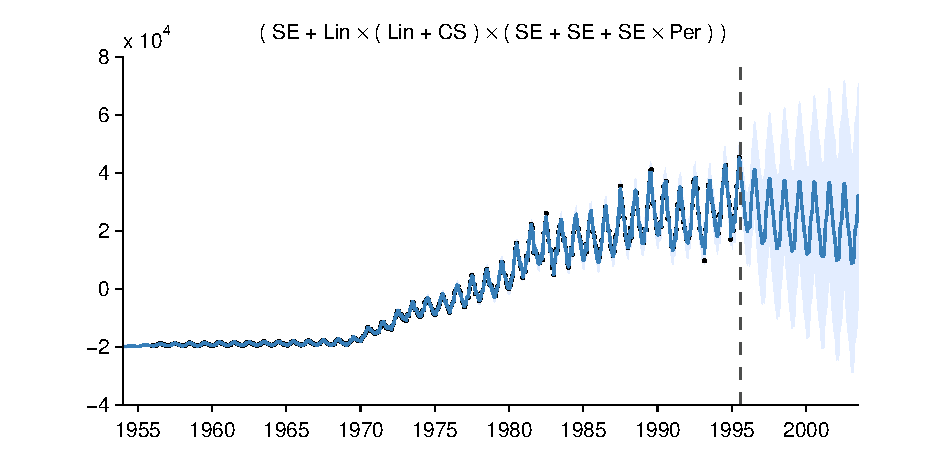
\includegraphics[width=\wmgd,height=\hmgd]{\mdrd/monthly-production-of-gas-in-aus_all} \\ = \\

\mbm 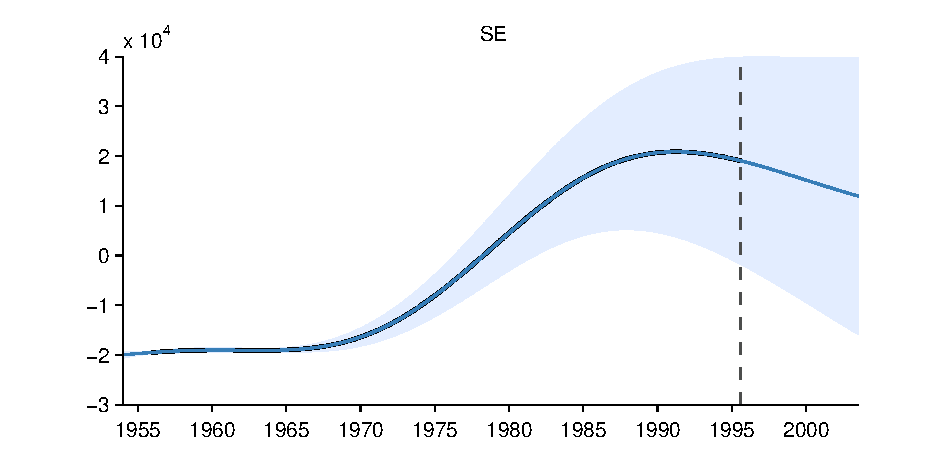
\includegraphics[width=\wmgd,height=\hmgd]{\mdrd/monthly-production-of-gas-in-aus_1} \\ + \\

\mbm 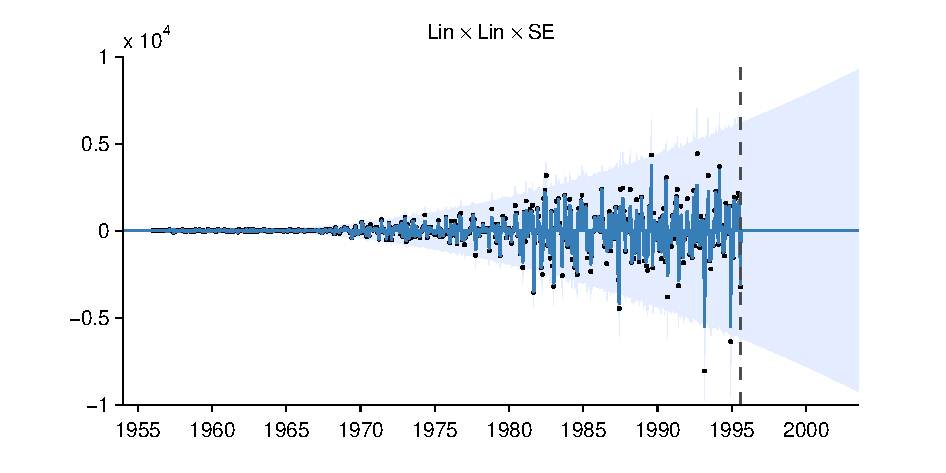
\includegraphics[width=\wmgd,height=\hmgd]{\mdrd/monthly-production-of-gas-in-aus_2} \\ + \\

\mbm 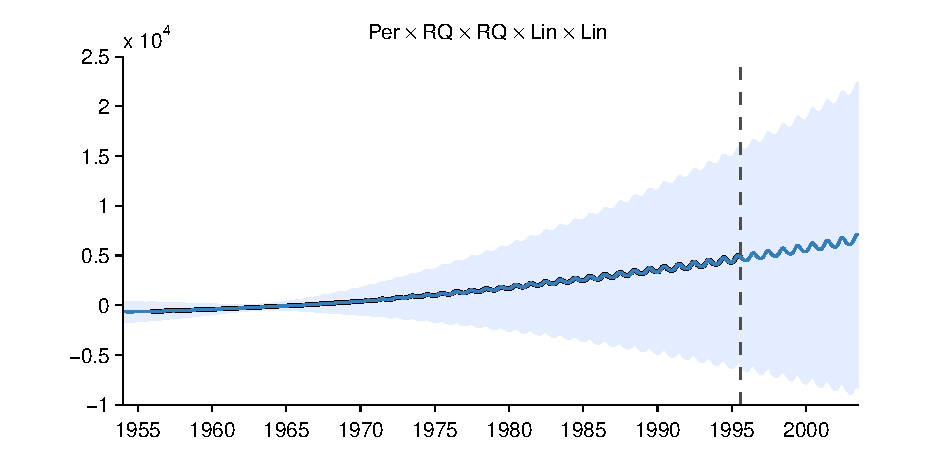
\includegraphics[width=\wmgd,height=\hmgd]{\mdrd/monthly-production-of-gas-in-aus_3} \\ + \\

\mbm 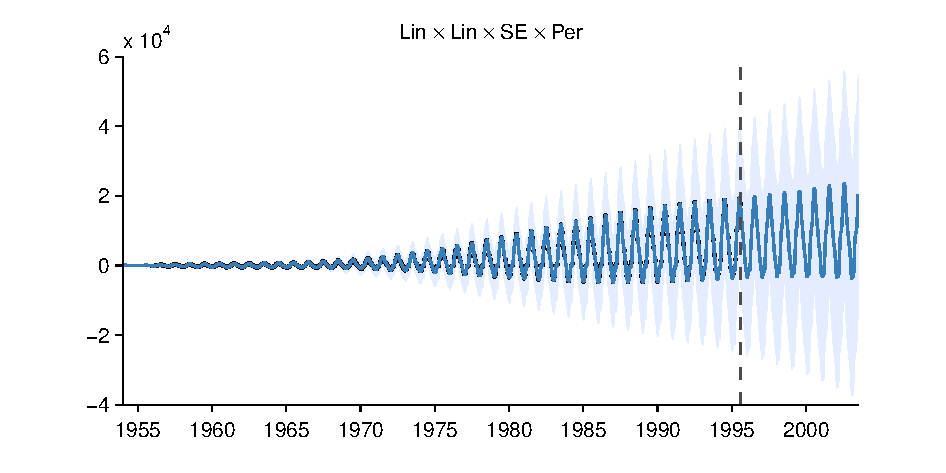
\includegraphics[width=\wmgd,height=\hmgd]{\mdrd/monthly-production-of-gas-in-aus_4} \\ + \\

\mbm 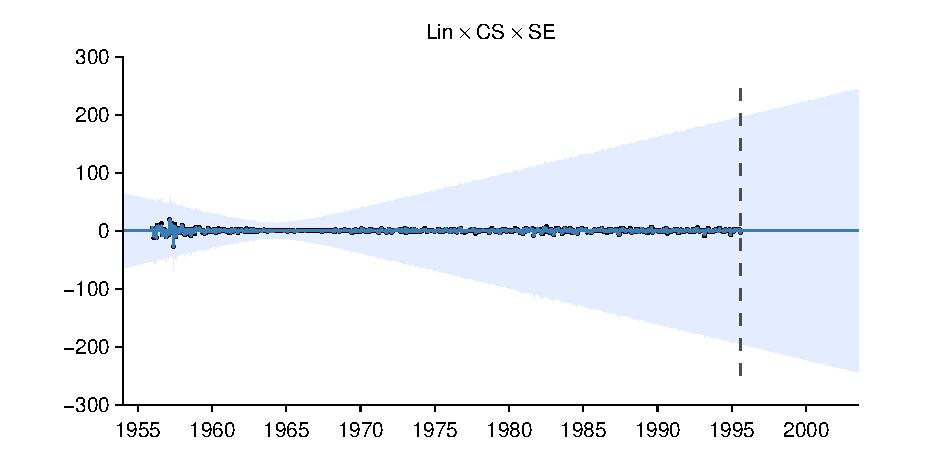
\includegraphics[width=\wmgd,height=\hmgd]{\mdrd/monthly-production-of-gas-in-aus_5} \\ + \\

\mbm 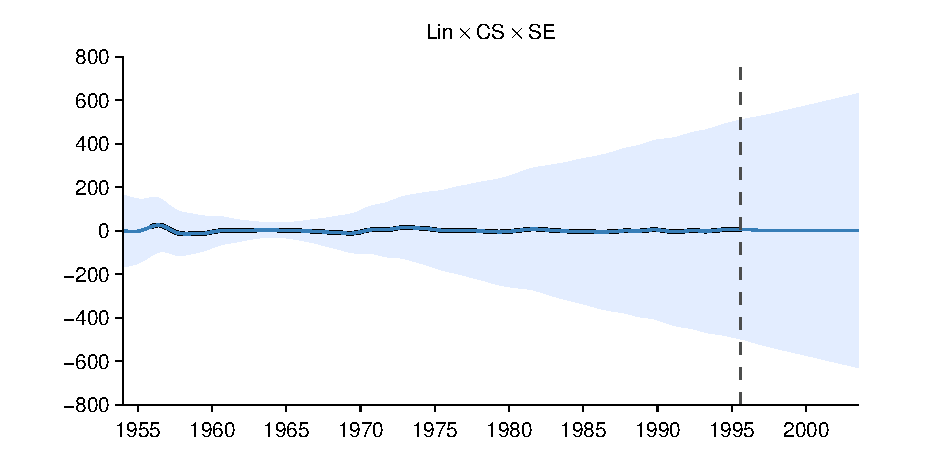
\includegraphics[width=\wmgd,height=\hmgd]{\mdrd/monthly-production-of-gas-in-aus_6} \\ + \\

\mbm 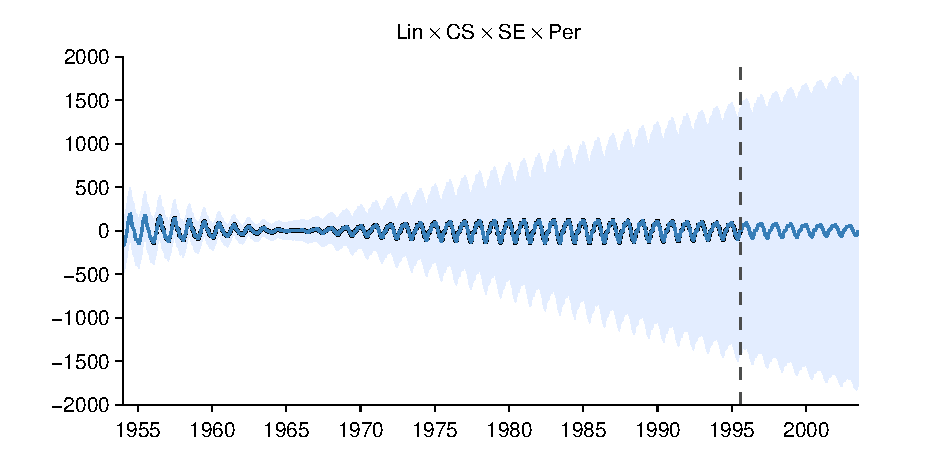
\includegraphics[width=\wmgd,height=\hmgd]{\mdrd/monthly-production-of-gas-in-aus_7} \\ + \\

\mbm 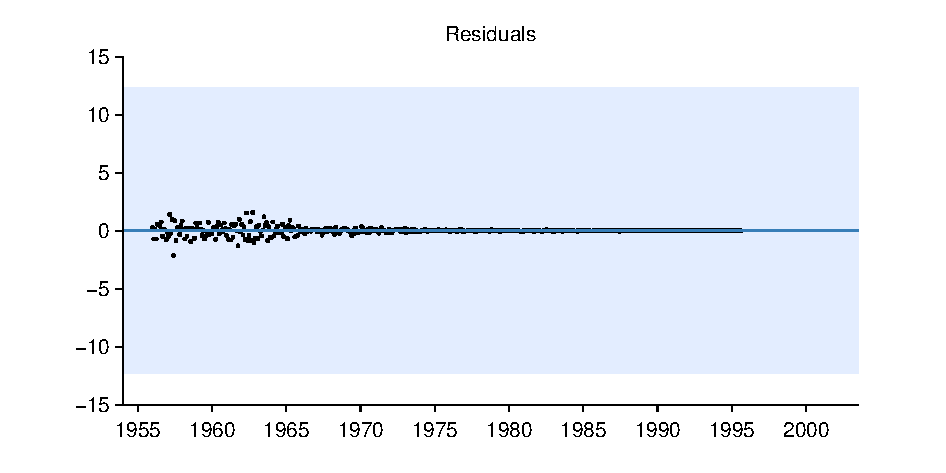
\includegraphics[width=\wmgd,height=\hmgd]{\mdrd/monthly-production-of-gas-in-aus_resid}
\end{tabular}
\end{figure}
    

\section{02-solar}


\begin{figure}[H]
\newcommand{\wmgd}{1\columnwidth}
\newcommand{\hmgd}{3.0cm}
\newcommand{\mdrd}{figures/monthly-production-of-gas-in-aus}
\newcommand{\mbm}{\hspace{-0.3cm}}
\begin{tabular}{c}
\mbm 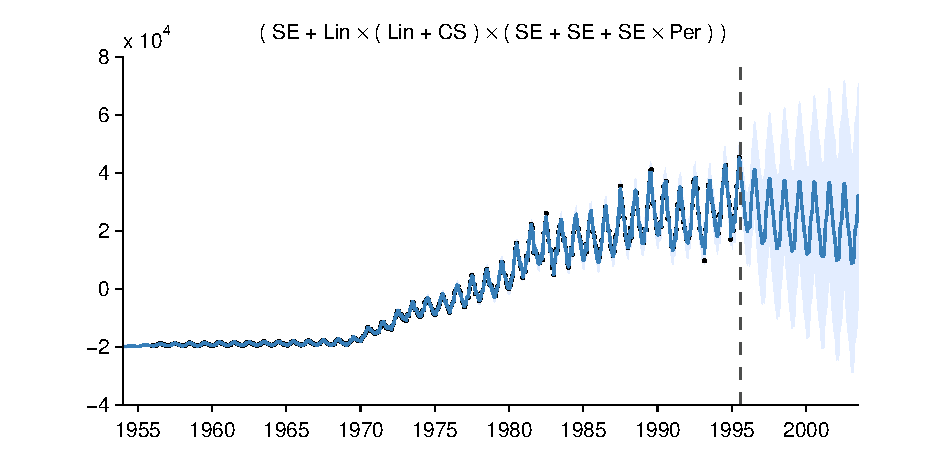
\includegraphics[width=\wmgd,height=\hmgd]{\mdrd/monthly-production-of-gas-in-aus_all} \\ = \\

\mbm 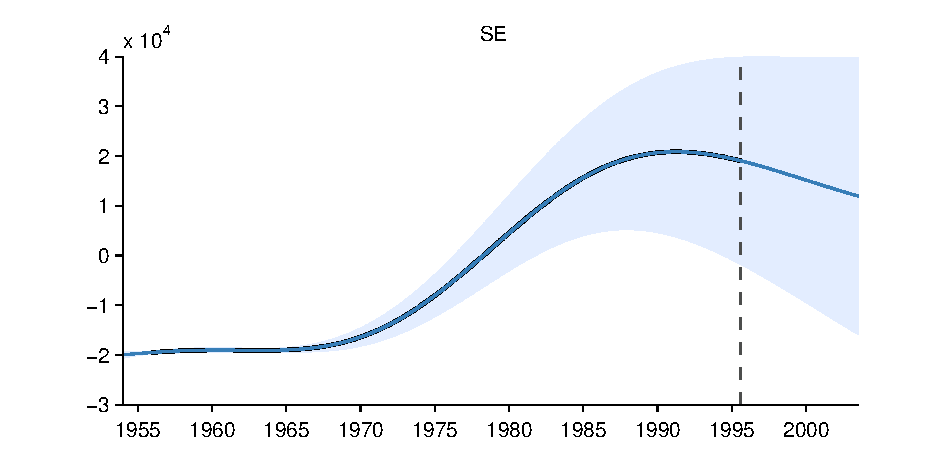
\includegraphics[width=\wmgd,height=\hmgd]{\mdrd/monthly-production-of-gas-in-aus_1} \\ + \\

\mbm 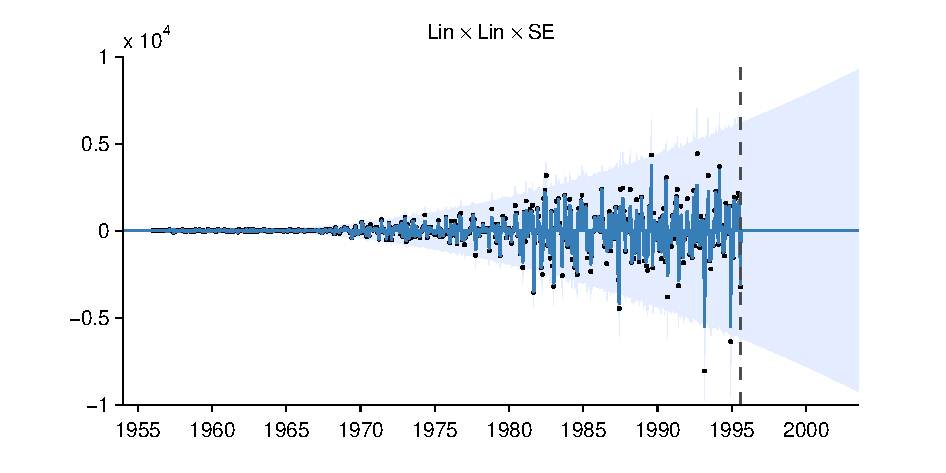
\includegraphics[width=\wmgd,height=\hmgd]{\mdrd/monthly-production-of-gas-in-aus_2} \\ + \\

\mbm 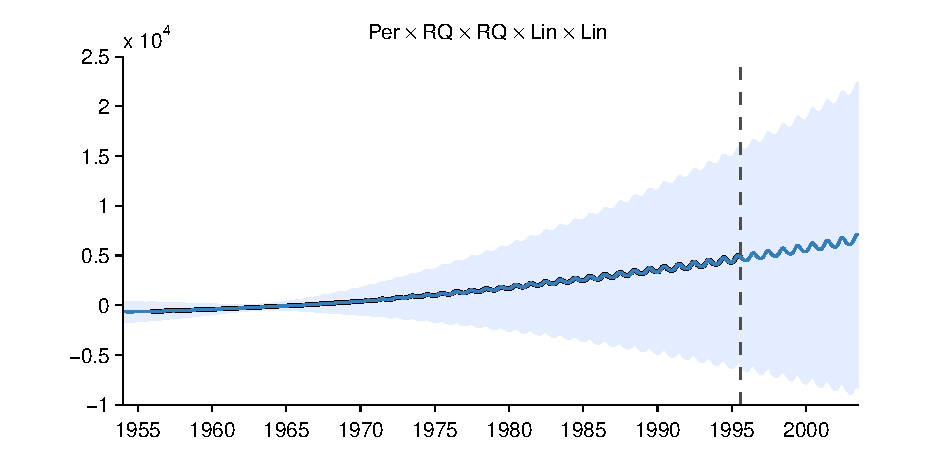
\includegraphics[width=\wmgd,height=\hmgd]{\mdrd/monthly-production-of-gas-in-aus_3} \\ + \\

\mbm 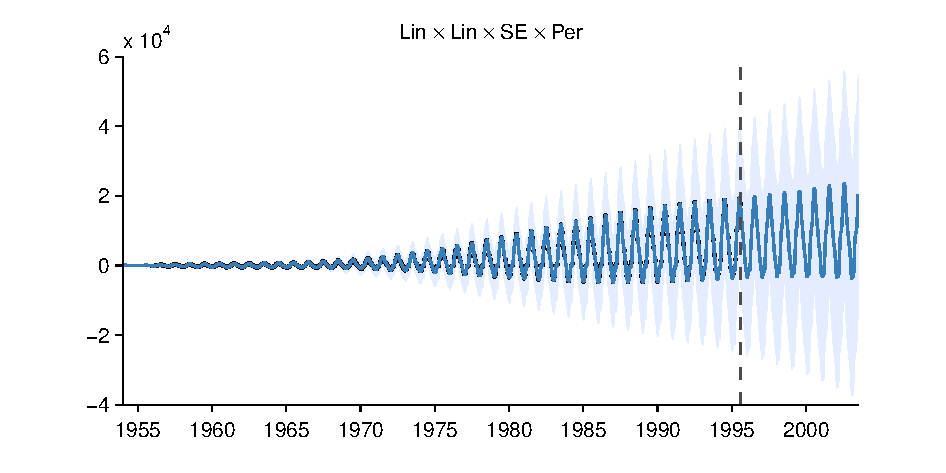
\includegraphics[width=\wmgd,height=\hmgd]{\mdrd/monthly-production-of-gas-in-aus_4} \\ + \\

\mbm 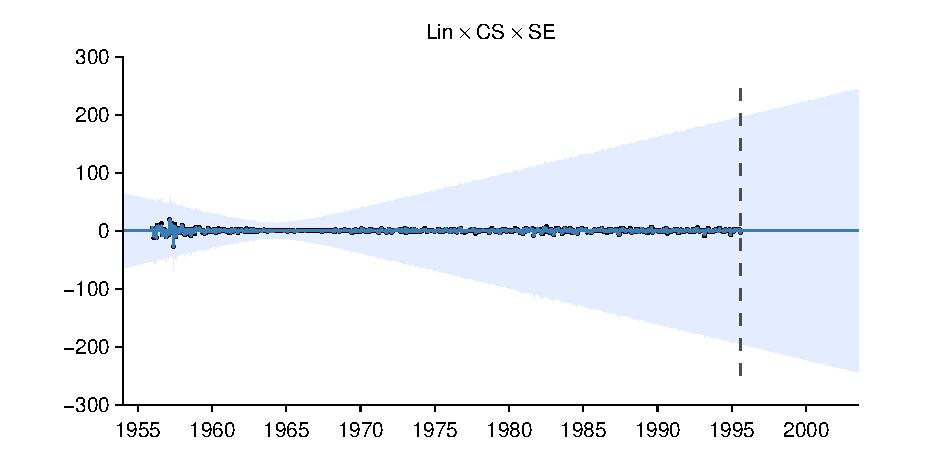
\includegraphics[width=\wmgd,height=\hmgd]{\mdrd/monthly-production-of-gas-in-aus_5} \\ + \\

\mbm 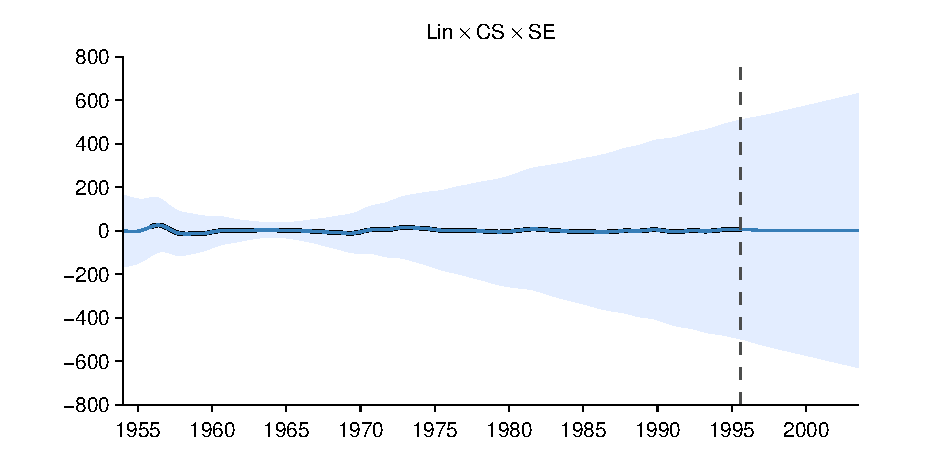
\includegraphics[width=\wmgd,height=\hmgd]{\mdrd/monthly-production-of-gas-in-aus_6} \\ + \\

\mbm 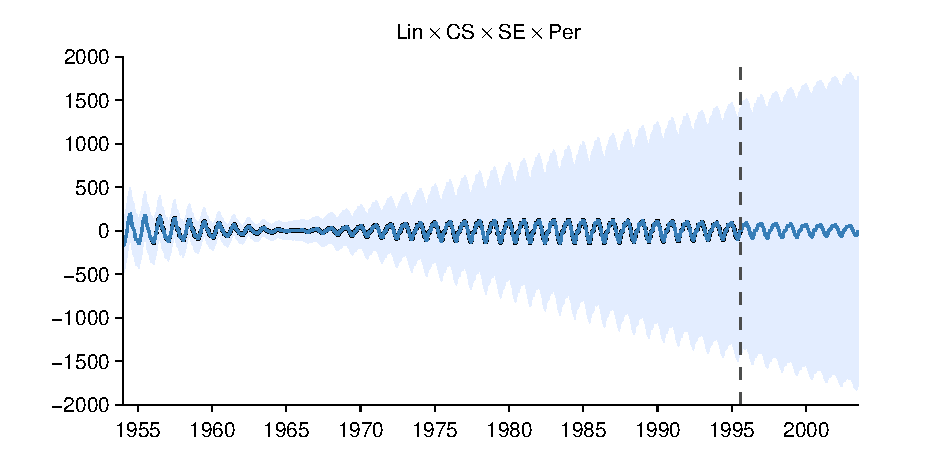
\includegraphics[width=\wmgd,height=\hmgd]{\mdrd/monthly-production-of-gas-in-aus_7} \\ + \\

\mbm 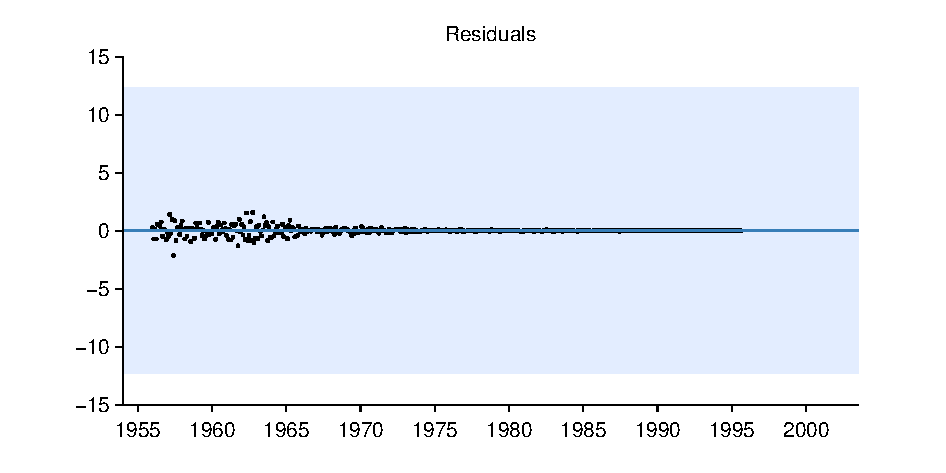
\includegraphics[width=\wmgd,height=\hmgd]{\mdrd/monthly-production-of-gas-in-aus_resid}
\end{tabular}
\end{figure}
    

\section{03-mauna2003}


\begin{figure}[H]
\newcommand{\wmgd}{1\columnwidth}
\newcommand{\hmgd}{3.0cm}
\newcommand{\mdrd}{figures/monthly-production-of-gas-in-aus}
\newcommand{\mbm}{\hspace{-0.3cm}}
\begin{tabular}{c}
\mbm 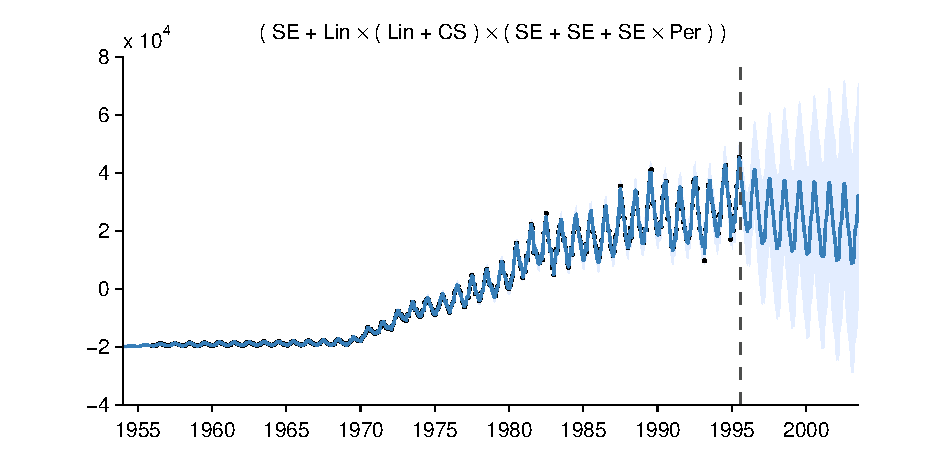
\includegraphics[width=\wmgd,height=\hmgd]{\mdrd/monthly-production-of-gas-in-aus_all} \\ = \\

\mbm 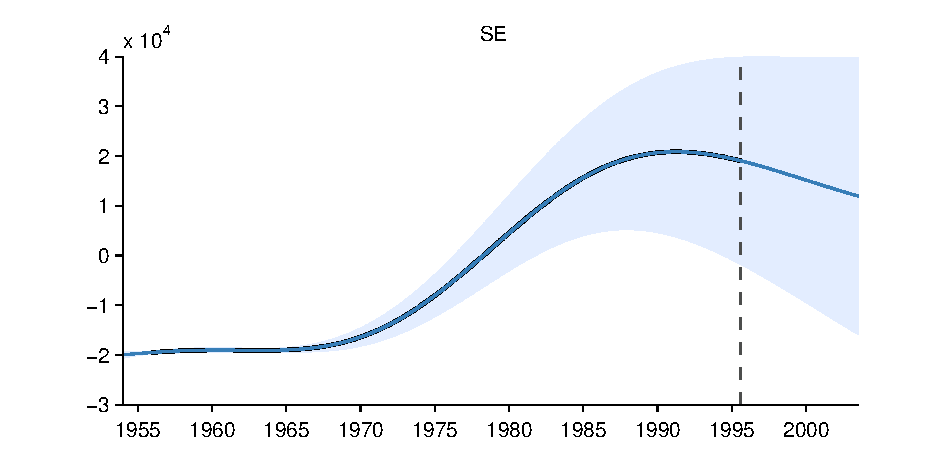
\includegraphics[width=\wmgd,height=\hmgd]{\mdrd/monthly-production-of-gas-in-aus_1} \\ + \\

\mbm 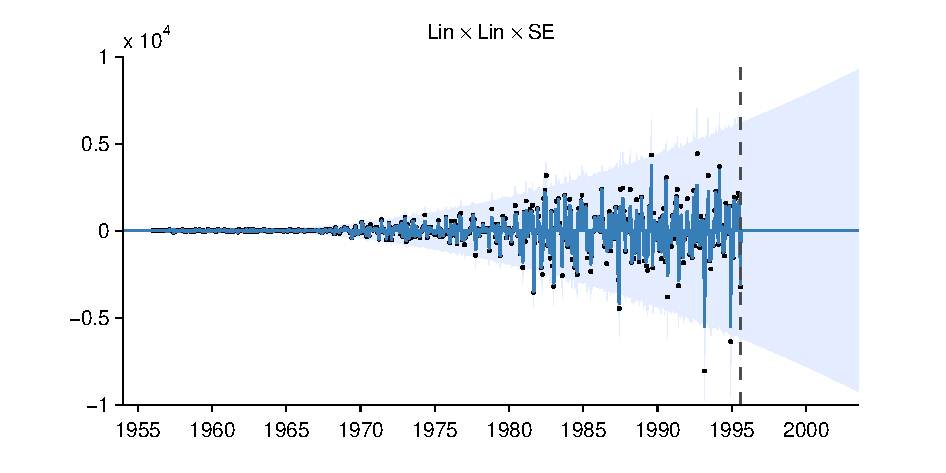
\includegraphics[width=\wmgd,height=\hmgd]{\mdrd/monthly-production-of-gas-in-aus_2} \\ + \\

\mbm 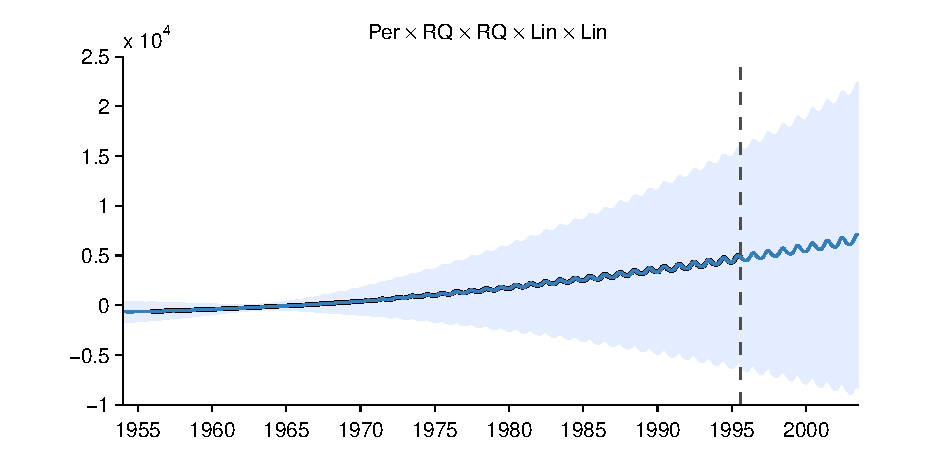
\includegraphics[width=\wmgd,height=\hmgd]{\mdrd/monthly-production-of-gas-in-aus_3} \\ + \\

\mbm 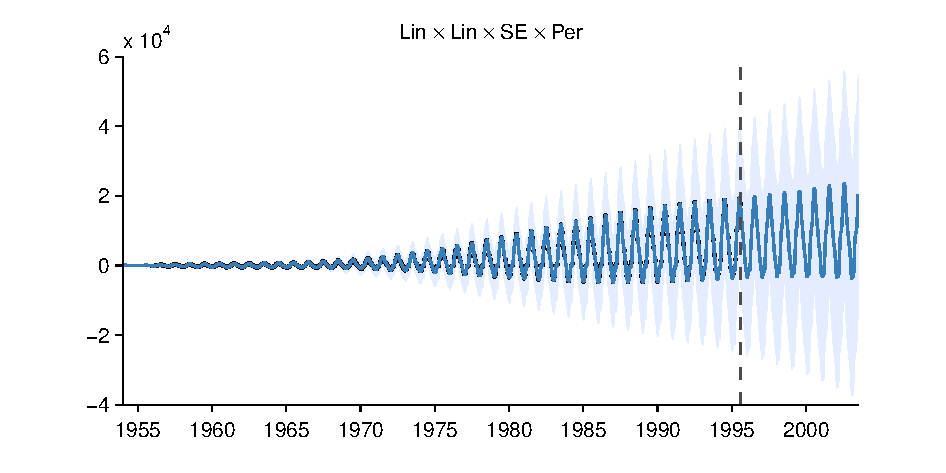
\includegraphics[width=\wmgd,height=\hmgd]{\mdrd/monthly-production-of-gas-in-aus_4} \\ + \\

\mbm 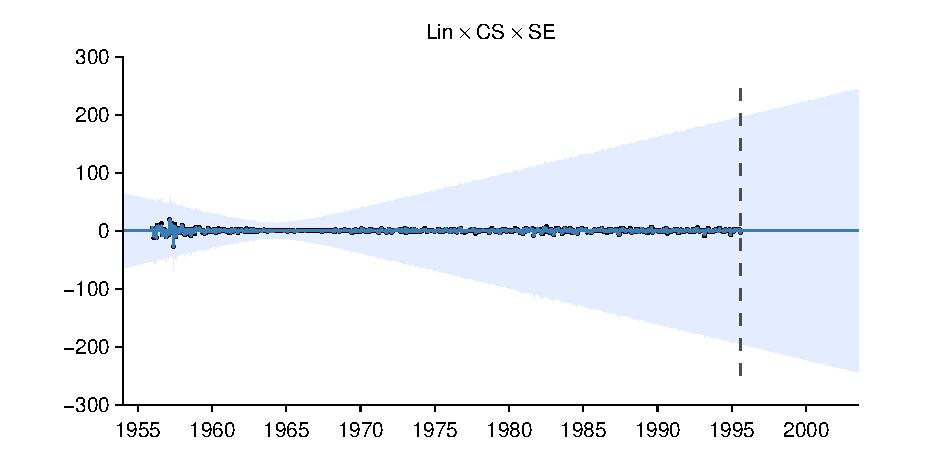
\includegraphics[width=\wmgd,height=\hmgd]{\mdrd/monthly-production-of-gas-in-aus_5} \\ + \\

\mbm 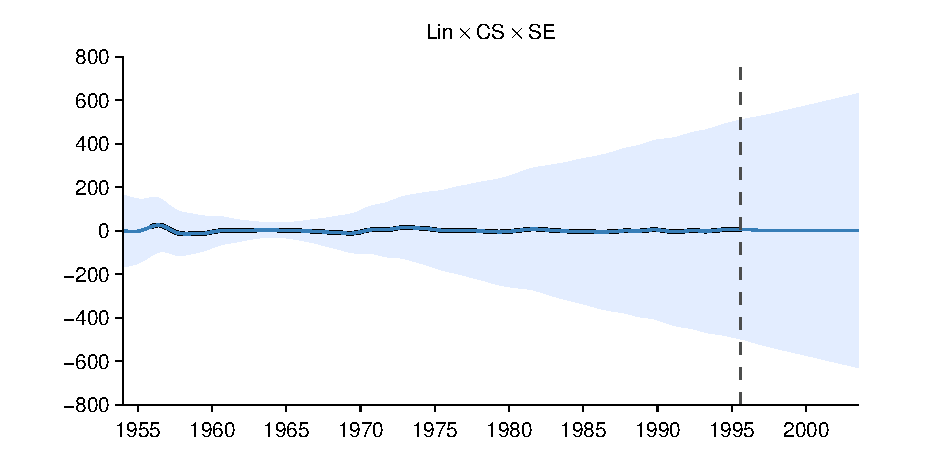
\includegraphics[width=\wmgd,height=\hmgd]{\mdrd/monthly-production-of-gas-in-aus_6} \\ + \\

\mbm 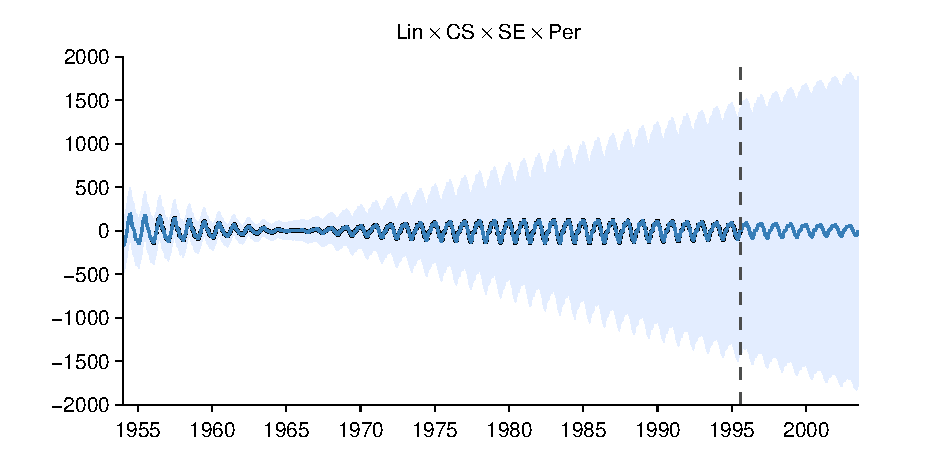
\includegraphics[width=\wmgd,height=\hmgd]{\mdrd/monthly-production-of-gas-in-aus_7} \\ + \\

\mbm 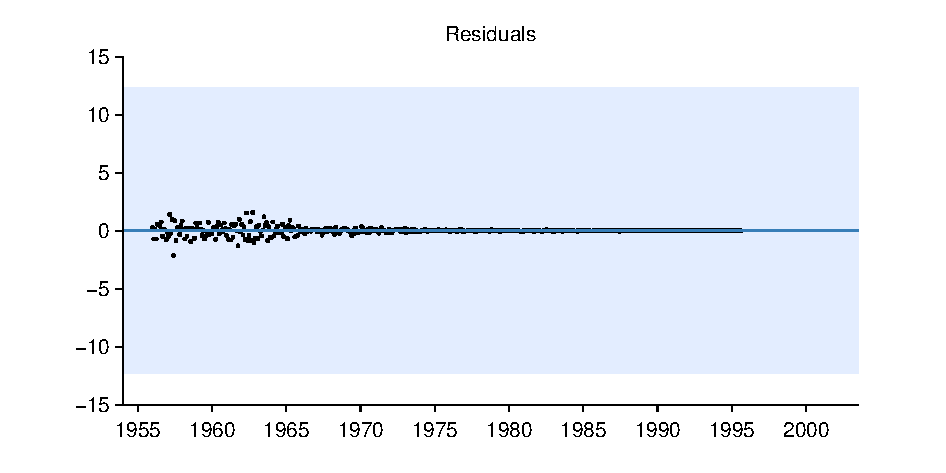
\includegraphics[width=\wmgd,height=\hmgd]{\mdrd/monthly-production-of-gas-in-aus_resid}
\end{tabular}
\end{figure}
    

\section{04-sea-level-mothly}


\begin{figure}[H]
\newcommand{\wmgd}{1\columnwidth}
\newcommand{\hmgd}{3.0cm}
\newcommand{\mdrd}{figures/monthly-production-of-gas-in-aus}
\newcommand{\mbm}{\hspace{-0.3cm}}
\begin{tabular}{c}
\mbm 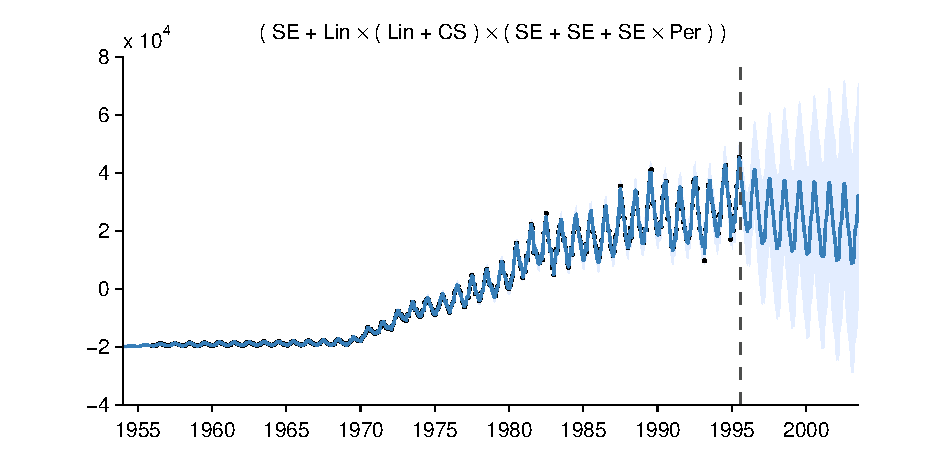
\includegraphics[width=\wmgd,height=\hmgd]{\mdrd/monthly-production-of-gas-in-aus_all} \\ = \\

\mbm 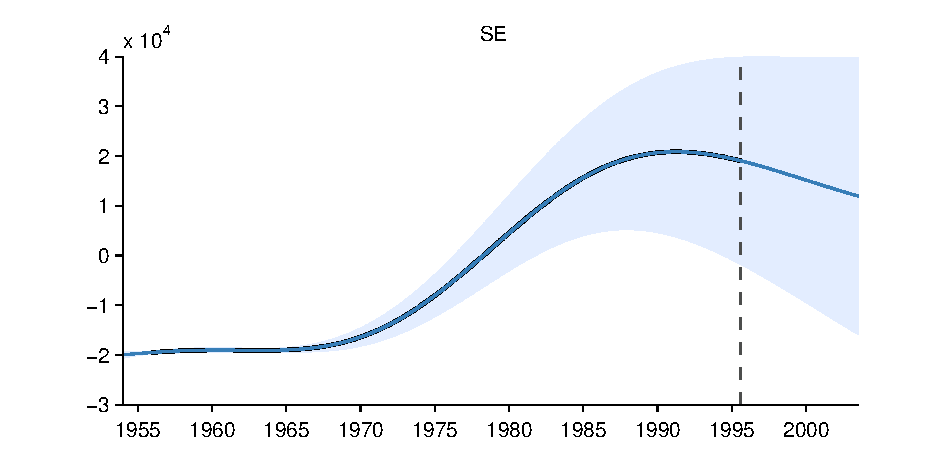
\includegraphics[width=\wmgd,height=\hmgd]{\mdrd/monthly-production-of-gas-in-aus_1} \\ + \\

\mbm 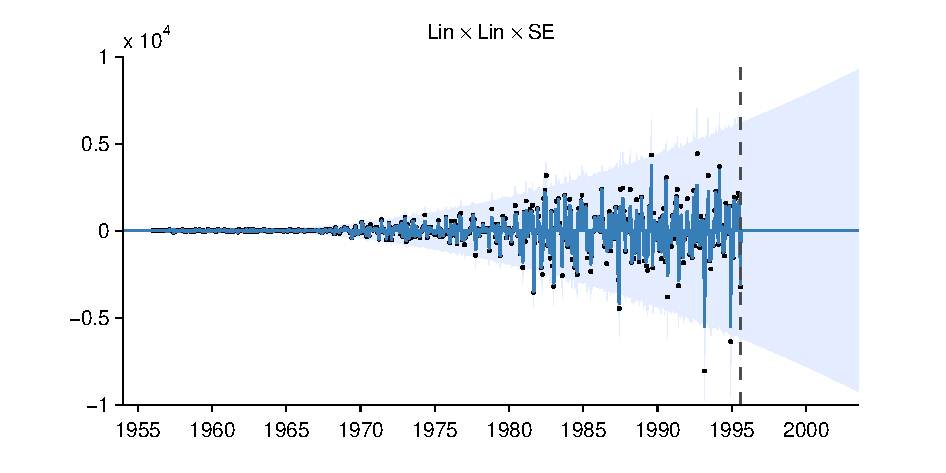
\includegraphics[width=\wmgd,height=\hmgd]{\mdrd/monthly-production-of-gas-in-aus_2} \\ + \\

\mbm 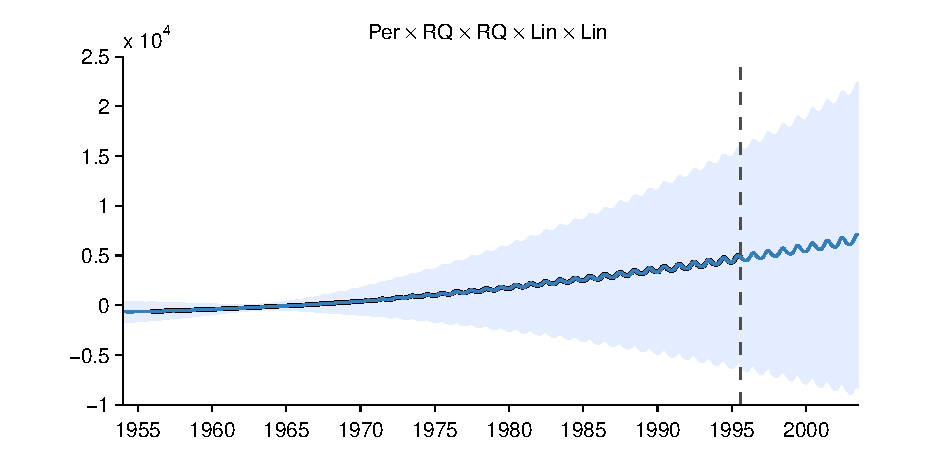
\includegraphics[width=\wmgd,height=\hmgd]{\mdrd/monthly-production-of-gas-in-aus_3} \\ + \\

\mbm 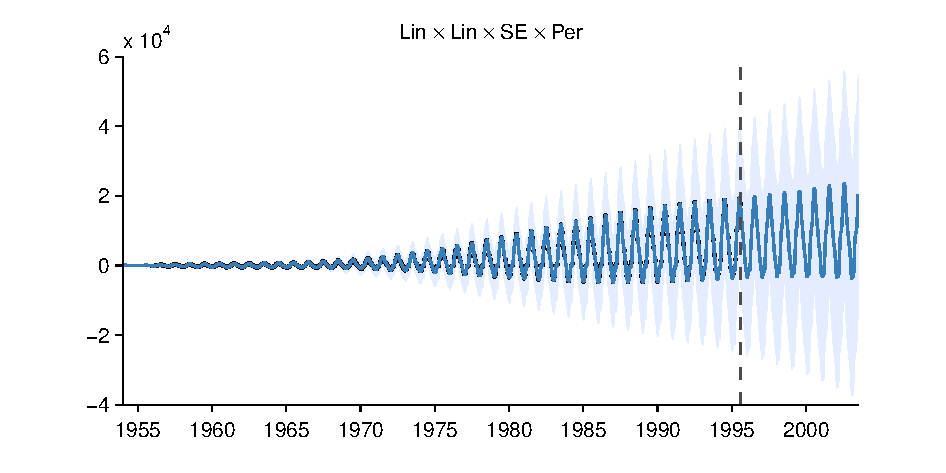
\includegraphics[width=\wmgd,height=\hmgd]{\mdrd/monthly-production-of-gas-in-aus_4} \\ + \\

\mbm 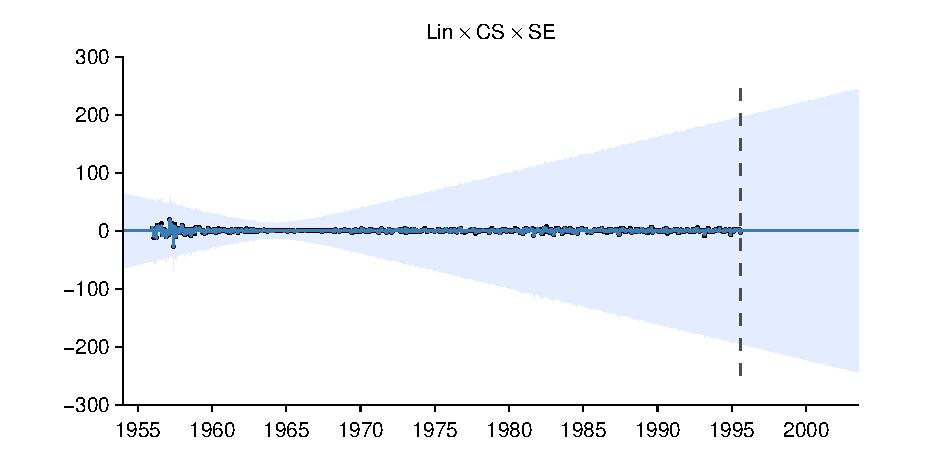
\includegraphics[width=\wmgd,height=\hmgd]{\mdrd/monthly-production-of-gas-in-aus_5} \\ + \\

\mbm 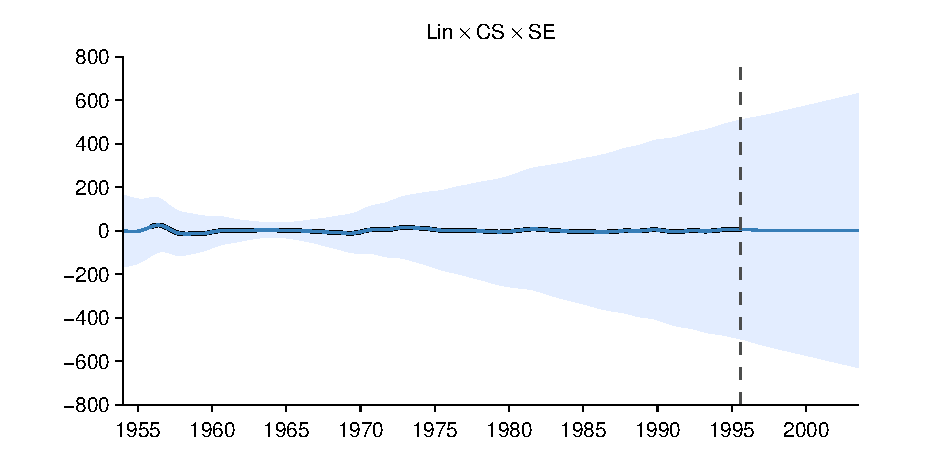
\includegraphics[width=\wmgd,height=\hmgd]{\mdrd/monthly-production-of-gas-in-aus_6} \\ + \\

\mbm 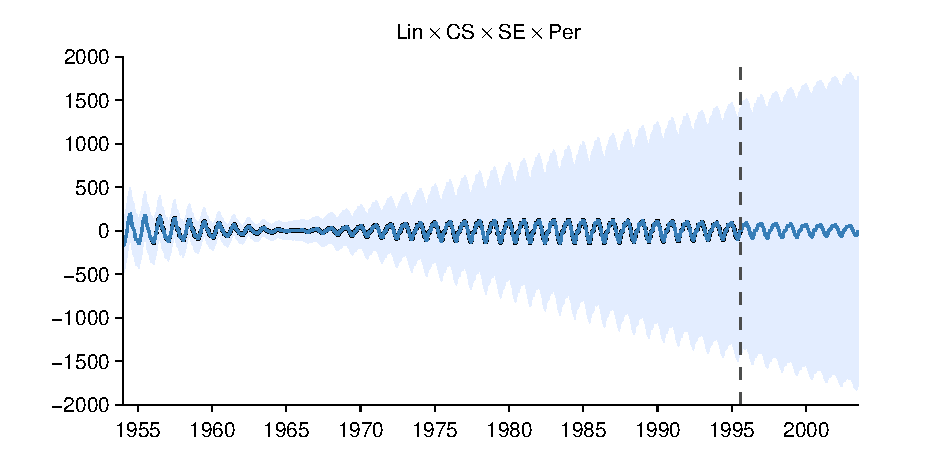
\includegraphics[width=\wmgd,height=\hmgd]{\mdrd/monthly-production-of-gas-in-aus_7} \\ + \\

\mbm 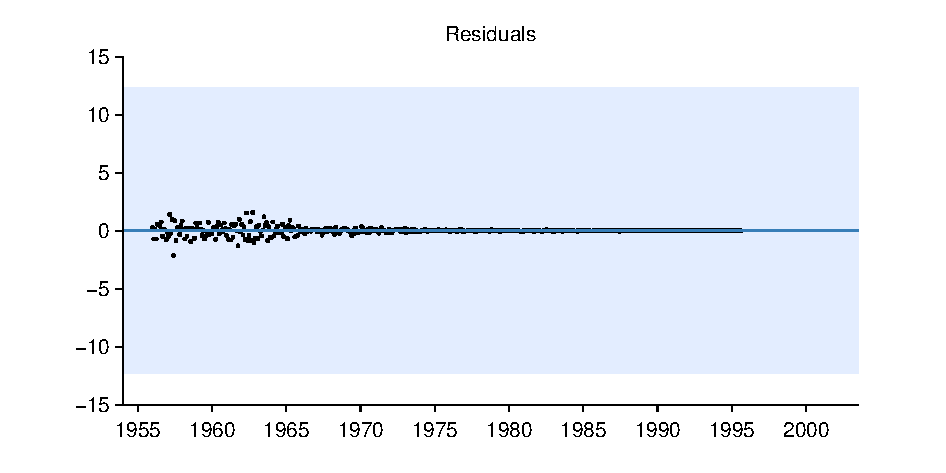
\includegraphics[width=\wmgd,height=\hmgd]{\mdrd/monthly-production-of-gas-in-aus_resid}
\end{tabular}
\end{figure}
    

\section{06-methane-750-thin}


\begin{figure}[H]
\newcommand{\wmgd}{1\columnwidth}
\newcommand{\hmgd}{3.0cm}
\newcommand{\mdrd}{figures/monthly-production-of-gas-in-aus}
\newcommand{\mbm}{\hspace{-0.3cm}}
\begin{tabular}{c}
\mbm 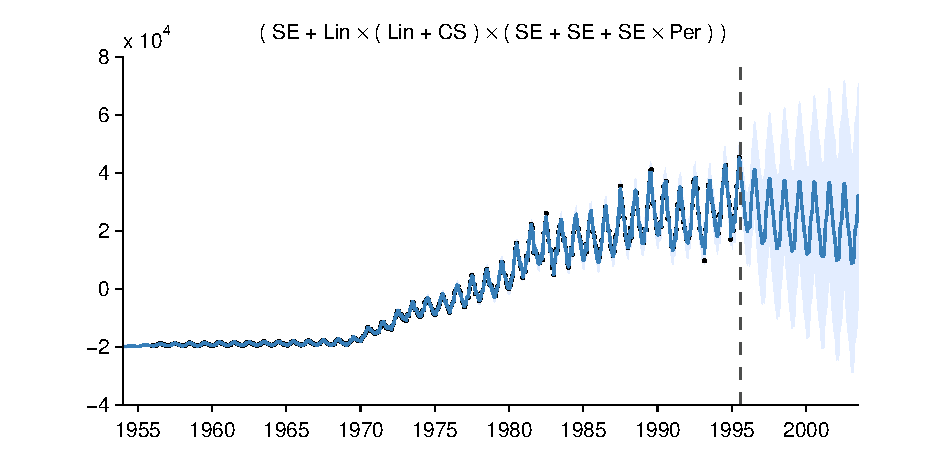
\includegraphics[width=\wmgd,height=\hmgd]{\mdrd/monthly-production-of-gas-in-aus_all} \\ = \\

\mbm 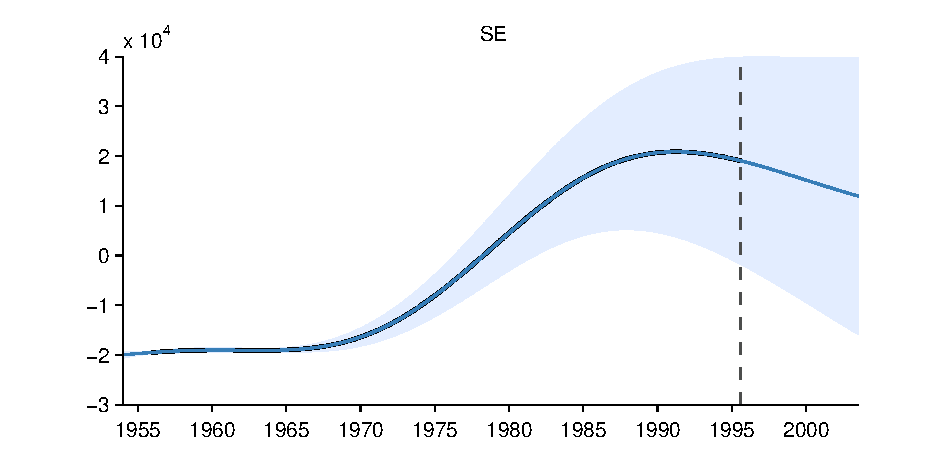
\includegraphics[width=\wmgd,height=\hmgd]{\mdrd/monthly-production-of-gas-in-aus_1} \\ + \\

\mbm 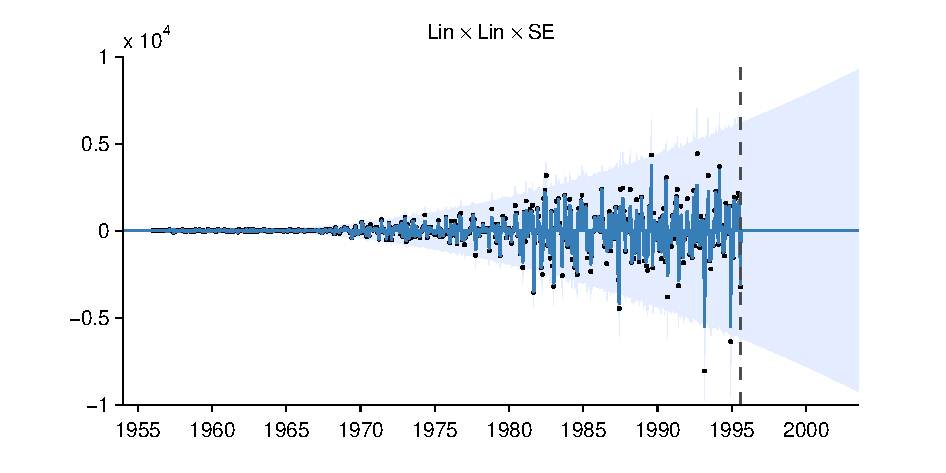
\includegraphics[width=\wmgd,height=\hmgd]{\mdrd/monthly-production-of-gas-in-aus_2} \\ + \\

\mbm 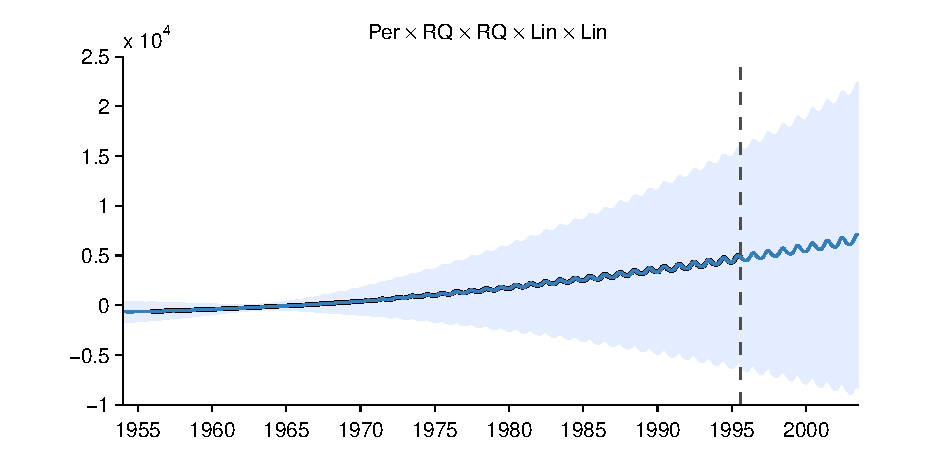
\includegraphics[width=\wmgd,height=\hmgd]{\mdrd/monthly-production-of-gas-in-aus_3} \\ + \\

\mbm 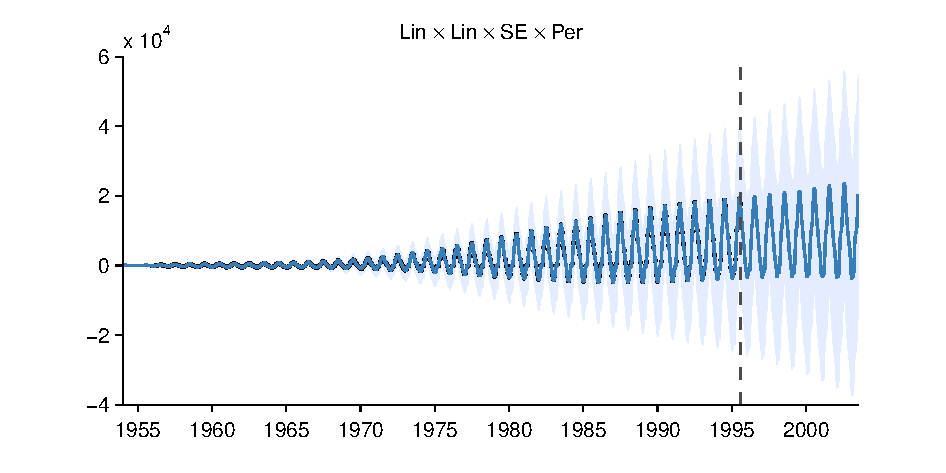
\includegraphics[width=\wmgd,height=\hmgd]{\mdrd/monthly-production-of-gas-in-aus_4} \\ + \\

\mbm 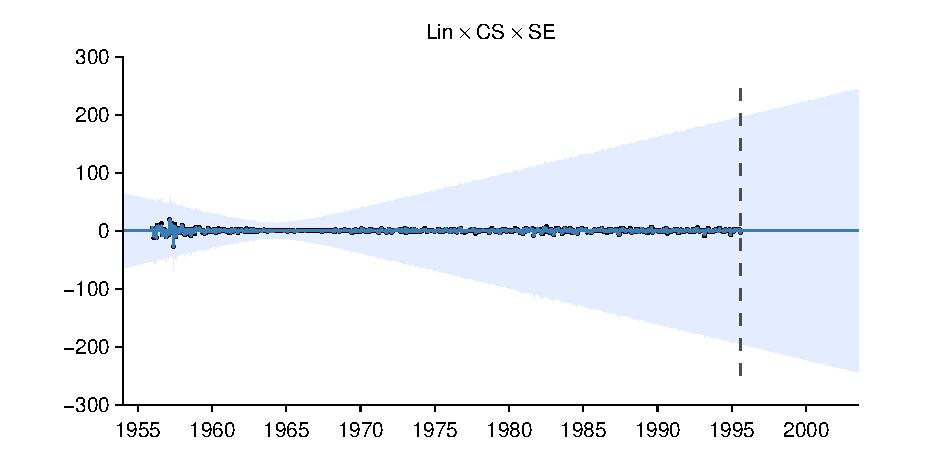
\includegraphics[width=\wmgd,height=\hmgd]{\mdrd/monthly-production-of-gas-in-aus_5} \\ + \\

\mbm 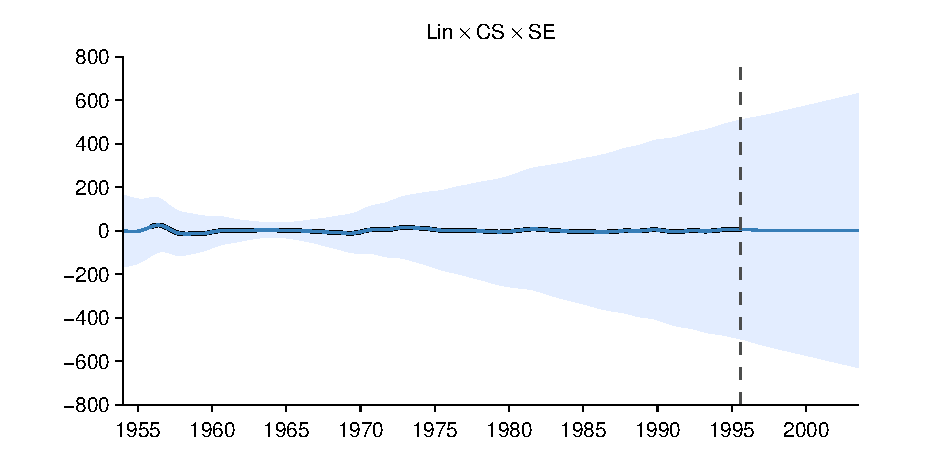
\includegraphics[width=\wmgd,height=\hmgd]{\mdrd/monthly-production-of-gas-in-aus_6} \\ + \\

\mbm 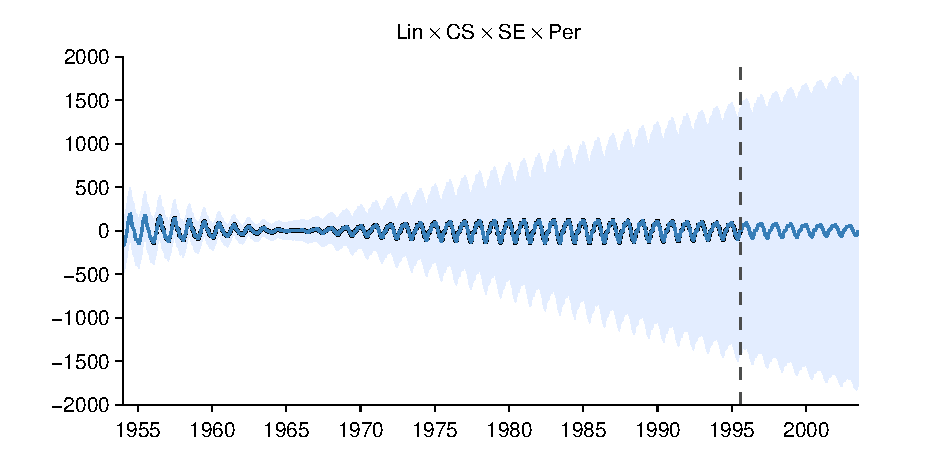
\includegraphics[width=\wmgd,height=\hmgd]{\mdrd/monthly-production-of-gas-in-aus_7} \\ + \\

\mbm 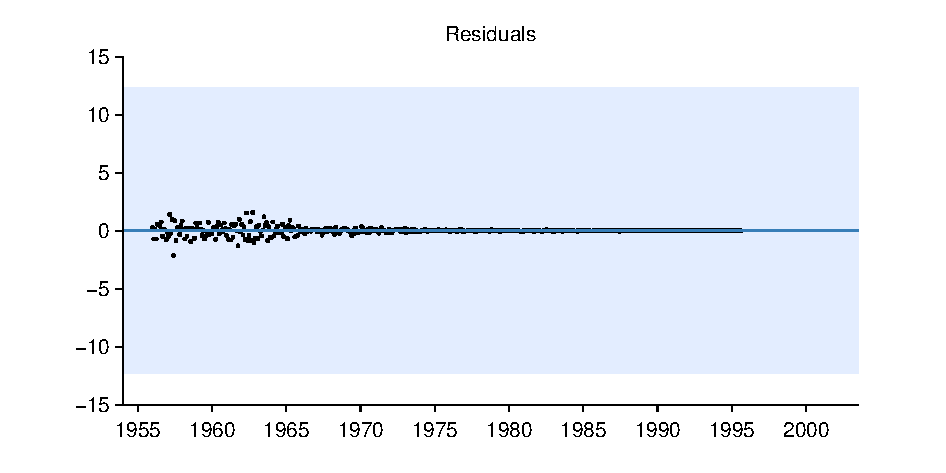
\includegraphics[width=\wmgd,height=\hmgd]{\mdrd/monthly-production-of-gas-in-aus_resid}
\end{tabular}
\end{figure}
    

\section{accidental-deaths-in-usa-monthly}


\begin{figure}[H]
\newcommand{\wmgd}{1\columnwidth}
\newcommand{\hmgd}{3.0cm}
\newcommand{\mdrd}{figures/monthly-production-of-gas-in-aus}
\newcommand{\mbm}{\hspace{-0.3cm}}
\begin{tabular}{c}
\mbm 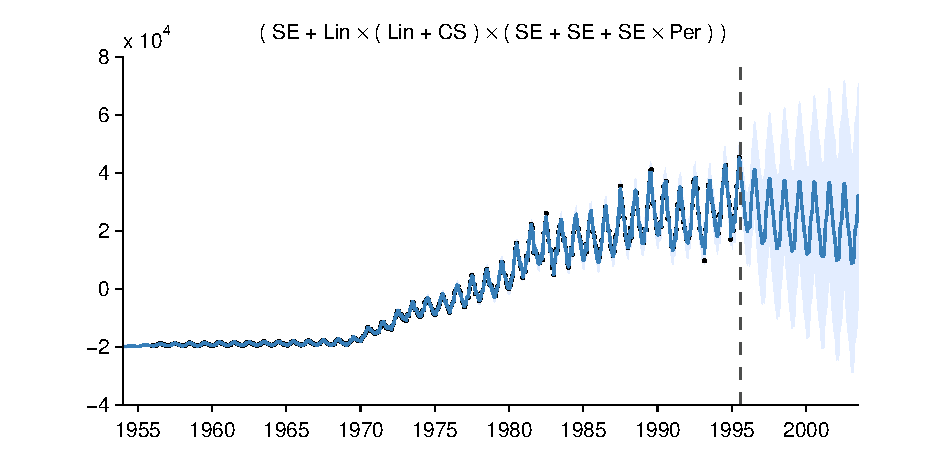
\includegraphics[width=\wmgd,height=\hmgd]{\mdrd/monthly-production-of-gas-in-aus_all} \\ = \\

\mbm 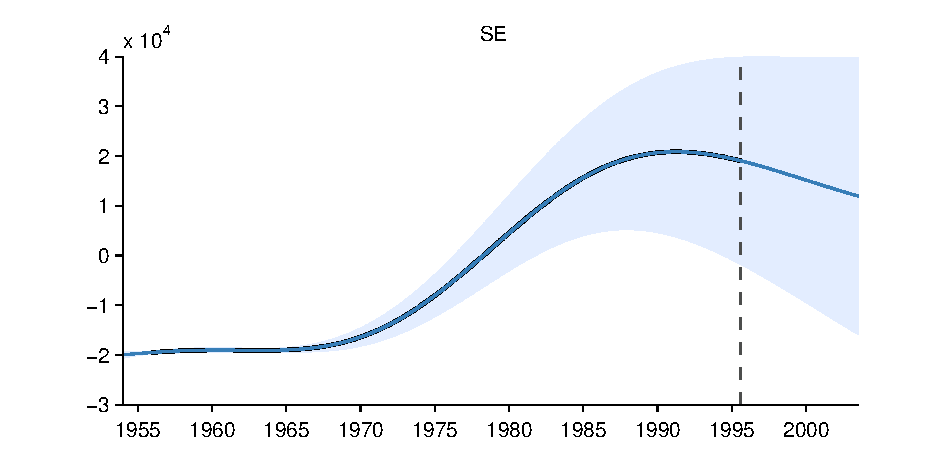
\includegraphics[width=\wmgd,height=\hmgd]{\mdrd/monthly-production-of-gas-in-aus_1} \\ + \\

\mbm 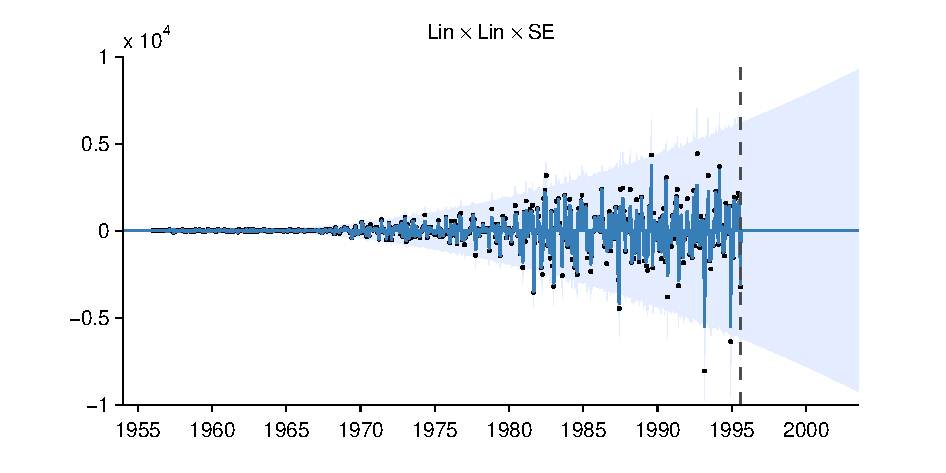
\includegraphics[width=\wmgd,height=\hmgd]{\mdrd/monthly-production-of-gas-in-aus_2} \\ + \\

\mbm 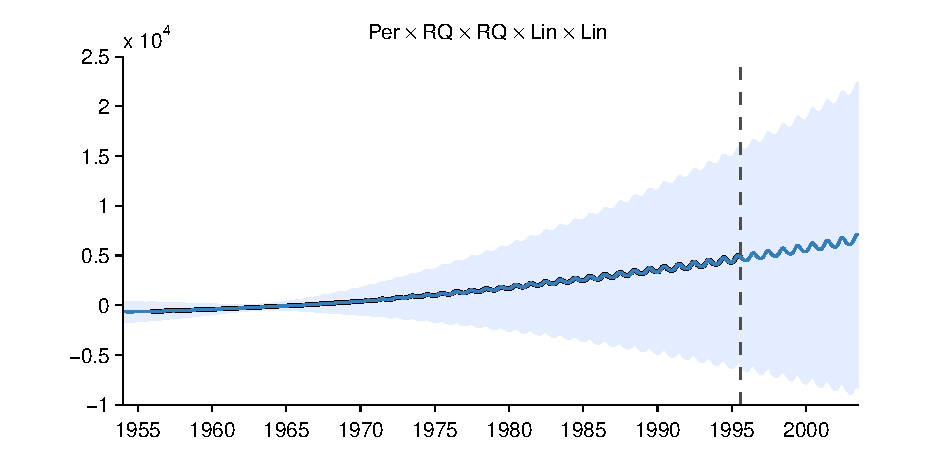
\includegraphics[width=\wmgd,height=\hmgd]{\mdrd/monthly-production-of-gas-in-aus_3} \\ + \\

\mbm 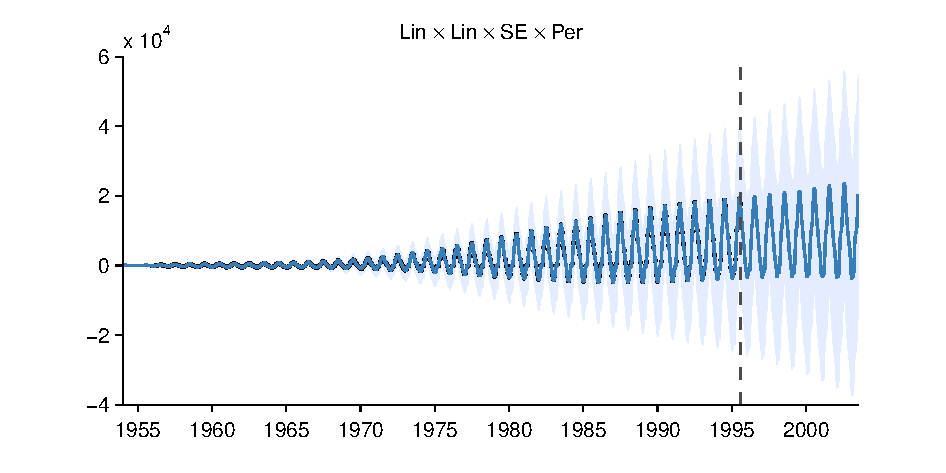
\includegraphics[width=\wmgd,height=\hmgd]{\mdrd/monthly-production-of-gas-in-aus_4} \\ + \\

\mbm \includegraphics[width=\wmgd,height=\hmgd]{\mdrd/monthly-production-of-gas-in-aus_5} \\ + \\

\mbm \includegraphics[width=\wmgd,height=\hmgd]{\mdrd/monthly-production-of-gas-in-aus_6} \\ + \\

\mbm \includegraphics[width=\wmgd,height=\hmgd]{\mdrd/monthly-production-of-gas-in-aus_7} \\ + \\

\mbm \includegraphics[width=\wmgd,height=\hmgd]{\mdrd/monthly-production-of-gas-in-aus_resid}
\end{tabular}
\end{figure}
    

\section{annual-number-of-lynx-trapped-ma}


\begin{figure}[H]
\newcommand{\wmgd}{1\columnwidth}
\newcommand{\hmgd}{3.0cm}
\newcommand{\mdrd}{figures/monthly-production-of-gas-in-aus}
\newcommand{\mbm}{\hspace{-0.3cm}}
\begin{tabular}{c}
\mbm \includegraphics[width=\wmgd,height=\hmgd]{\mdrd/monthly-production-of-gas-in-aus_all} \\ = \\

\mbm \includegraphics[width=\wmgd,height=\hmgd]{\mdrd/monthly-production-of-gas-in-aus_1} \\ + \\

\mbm \includegraphics[width=\wmgd,height=\hmgd]{\mdrd/monthly-production-of-gas-in-aus_2} \\ + \\

\mbm \includegraphics[width=\wmgd,height=\hmgd]{\mdrd/monthly-production-of-gas-in-aus_3} \\ + \\

\mbm \includegraphics[width=\wmgd,height=\hmgd]{\mdrd/monthly-production-of-gas-in-aus_4} \\ + \\

\mbm \includegraphics[width=\wmgd,height=\hmgd]{\mdrd/monthly-production-of-gas-in-aus_5} \\ + \\

\mbm \includegraphics[width=\wmgd,height=\hmgd]{\mdrd/monthly-production-of-gas-in-aus_6} \\ + \\

\mbm \includegraphics[width=\wmgd,height=\hmgd]{\mdrd/monthly-production-of-gas-in-aus_7} \\ + \\

\mbm \includegraphics[width=\wmgd,height=\hmgd]{\mdrd/monthly-production-of-gas-in-aus_resid}
\end{tabular}
\end{figure}
    

\section{annual-swedish-fertility-rates-1}


\begin{figure}[H]
\newcommand{\wmgd}{1\columnwidth}
\newcommand{\hmgd}{3.0cm}
\newcommand{\mdrd}{figures/monthly-production-of-gas-in-aus}
\newcommand{\mbm}{\hspace{-0.3cm}}
\begin{tabular}{c}
\mbm \includegraphics[width=\wmgd,height=\hmgd]{\mdrd/monthly-production-of-gas-in-aus_all} \\ = \\

\mbm \includegraphics[width=\wmgd,height=\hmgd]{\mdrd/monthly-production-of-gas-in-aus_1} \\ + \\

\mbm \includegraphics[width=\wmgd,height=\hmgd]{\mdrd/monthly-production-of-gas-in-aus_2} \\ + \\

\mbm \includegraphics[width=\wmgd,height=\hmgd]{\mdrd/monthly-production-of-gas-in-aus_3} \\ + \\

\mbm \includegraphics[width=\wmgd,height=\hmgd]{\mdrd/monthly-production-of-gas-in-aus_4} \\ + \\

\mbm \includegraphics[width=\wmgd,height=\hmgd]{\mdrd/monthly-production-of-gas-in-aus_5} \\ + \\

\mbm \includegraphics[width=\wmgd,height=\hmgd]{\mdrd/monthly-production-of-gas-in-aus_6} \\ + \\

\mbm \includegraphics[width=\wmgd,height=\hmgd]{\mdrd/monthly-production-of-gas-in-aus_7} \\ + \\

\mbm \includegraphics[width=\wmgd,height=\hmgd]{\mdrd/monthly-production-of-gas-in-aus_resid}
\end{tabular}
\end{figure}
    

\section{annual-velocity-of-money-1869-to}


\begin{figure}[H]
\newcommand{\wmgd}{1\columnwidth}
\newcommand{\hmgd}{3.0cm}
\newcommand{\mdrd}{figures/monthly-production-of-gas-in-aus}
\newcommand{\mbm}{\hspace{-0.3cm}}
\begin{tabular}{c}
\mbm \includegraphics[width=\wmgd,height=\hmgd]{\mdrd/monthly-production-of-gas-in-aus_all} \\ = \\

\mbm \includegraphics[width=\wmgd,height=\hmgd]{\mdrd/monthly-production-of-gas-in-aus_1} \\ + \\

\mbm \includegraphics[width=\wmgd,height=\hmgd]{\mdrd/monthly-production-of-gas-in-aus_2} \\ + \\

\mbm \includegraphics[width=\wmgd,height=\hmgd]{\mdrd/monthly-production-of-gas-in-aus_3} \\ + \\

\mbm \includegraphics[width=\wmgd,height=\hmgd]{\mdrd/monthly-production-of-gas-in-aus_4} \\ + \\

\mbm \includegraphics[width=\wmgd,height=\hmgd]{\mdrd/monthly-production-of-gas-in-aus_5} \\ + \\

\mbm \includegraphics[width=\wmgd,height=\hmgd]{\mdrd/monthly-production-of-gas-in-aus_6} \\ + \\

\mbm \includegraphics[width=\wmgd,height=\hmgd]{\mdrd/monthly-production-of-gas-in-aus_7} \\ + \\

\mbm \includegraphics[width=\wmgd,height=\hmgd]{\mdrd/monthly-production-of-gas-in-aus_resid}
\end{tabular}
\end{figure}
    

\section{beveridge-wheat-price-index-1500}


\begin{figure}[H]
\newcommand{\wmgd}{1\columnwidth}
\newcommand{\hmgd}{3.0cm}
\newcommand{\mdrd}{figures/monthly-production-of-gas-in-aus}
\newcommand{\mbm}{\hspace{-0.3cm}}
\begin{tabular}{c}
\mbm \includegraphics[width=\wmgd,height=\hmgd]{\mdrd/monthly-production-of-gas-in-aus_all} \\ = \\

\mbm \includegraphics[width=\wmgd,height=\hmgd]{\mdrd/monthly-production-of-gas-in-aus_1} \\ + \\

\mbm \includegraphics[width=\wmgd,height=\hmgd]{\mdrd/monthly-production-of-gas-in-aus_2} \\ + \\

\mbm \includegraphics[width=\wmgd,height=\hmgd]{\mdrd/monthly-production-of-gas-in-aus_3} \\ + \\

\mbm \includegraphics[width=\wmgd,height=\hmgd]{\mdrd/monthly-production-of-gas-in-aus_4} \\ + \\

\mbm \includegraphics[width=\wmgd,height=\hmgd]{\mdrd/monthly-production-of-gas-in-aus_5} \\ + \\

\mbm \includegraphics[width=\wmgd,height=\hmgd]{\mdrd/monthly-production-of-gas-in-aus_6} \\ + \\

\mbm \includegraphics[width=\wmgd,height=\hmgd]{\mdrd/monthly-production-of-gas-in-aus_7} \\ + \\

\mbm \includegraphics[width=\wmgd,height=\hmgd]{\mdrd/monthly-production-of-gas-in-aus_resid}
\end{tabular}
\end{figure}
    

\section{daily-minimum-temperatures-in-me}


\begin{figure}[H]
\newcommand{\wmgd}{1\columnwidth}
\newcommand{\hmgd}{3.0cm}
\newcommand{\mdrd}{figures/monthly-production-of-gas-in-aus}
\newcommand{\mbm}{\hspace{-0.3cm}}
\begin{tabular}{c}
\mbm \includegraphics[width=\wmgd,height=\hmgd]{\mdrd/monthly-production-of-gas-in-aus_all} \\ = \\

\mbm \includegraphics[width=\wmgd,height=\hmgd]{\mdrd/monthly-production-of-gas-in-aus_1} \\ + \\

\mbm \includegraphics[width=\wmgd,height=\hmgd]{\mdrd/monthly-production-of-gas-in-aus_2} \\ + \\

\mbm \includegraphics[width=\wmgd,height=\hmgd]{\mdrd/monthly-production-of-gas-in-aus_3} \\ + \\

\mbm \includegraphics[width=\wmgd,height=\hmgd]{\mdrd/monthly-production-of-gas-in-aus_4} \\ + \\

\mbm \includegraphics[width=\wmgd,height=\hmgd]{\mdrd/monthly-production-of-gas-in-aus_5} \\ + \\

\mbm \includegraphics[width=\wmgd,height=\hmgd]{\mdrd/monthly-production-of-gas-in-aus_6} \\ + \\

\mbm \includegraphics[width=\wmgd,height=\hmgd]{\mdrd/monthly-production-of-gas-in-aus_7} \\ + \\

\mbm \includegraphics[width=\wmgd,height=\hmgd]{\mdrd/monthly-production-of-gas-in-aus_resid}
\end{tabular}
\end{figure}
    

\section{daily-total-female-births-in-cal}


\begin{figure}[H]
\newcommand{\wmgd}{1\columnwidth}
\newcommand{\hmgd}{3.0cm}
\newcommand{\mdrd}{figures/monthly-production-of-gas-in-aus}
\newcommand{\mbm}{\hspace{-0.3cm}}
\begin{tabular}{c}
\mbm \includegraphics[width=\wmgd,height=\hmgd]{\mdrd/monthly-production-of-gas-in-aus_all} \\ = \\

\mbm \includegraphics[width=\wmgd,height=\hmgd]{\mdrd/monthly-production-of-gas-in-aus_1} \\ + \\

\mbm \includegraphics[width=\wmgd,height=\hmgd]{\mdrd/monthly-production-of-gas-in-aus_2} \\ + \\

\mbm \includegraphics[width=\wmgd,height=\hmgd]{\mdrd/monthly-production-of-gas-in-aus_3} \\ + \\

\mbm \includegraphics[width=\wmgd,height=\hmgd]{\mdrd/monthly-production-of-gas-in-aus_4} \\ + \\

\mbm \includegraphics[width=\wmgd,height=\hmgd]{\mdrd/monthly-production-of-gas-in-aus_5} \\ + \\

\mbm \includegraphics[width=\wmgd,height=\hmgd]{\mdrd/monthly-production-of-gas-in-aus_6} \\ + \\

\mbm \includegraphics[width=\wmgd,height=\hmgd]{\mdrd/monthly-production-of-gas-in-aus_7} \\ + \\

\mbm \includegraphics[width=\wmgd,height=\hmgd]{\mdrd/monthly-production-of-gas-in-aus_resid}
\end{tabular}
\end{figure}
    

\section{fur-sales-mink-h-b-co-18481911}


\begin{figure}[H]
\newcommand{\wmgd}{1\columnwidth}
\newcommand{\hmgd}{3.0cm}
\newcommand{\mdrd}{figures/monthly-production-of-gas-in-aus}
\newcommand{\mbm}{\hspace{-0.3cm}}
\begin{tabular}{c}
\mbm \includegraphics[width=\wmgd,height=\hmgd]{\mdrd/monthly-production-of-gas-in-aus_all} \\ = \\

\mbm \includegraphics[width=\wmgd,height=\hmgd]{\mdrd/monthly-production-of-gas-in-aus_1} \\ + \\

\mbm \includegraphics[width=\wmgd,height=\hmgd]{\mdrd/monthly-production-of-gas-in-aus_2} \\ + \\

\mbm \includegraphics[width=\wmgd,height=\hmgd]{\mdrd/monthly-production-of-gas-in-aus_3} \\ + \\

\mbm \includegraphics[width=\wmgd,height=\hmgd]{\mdrd/monthly-production-of-gas-in-aus_4} \\ + \\

\mbm \includegraphics[width=\wmgd,height=\hmgd]{\mdrd/monthly-production-of-gas-in-aus_5} \\ + \\

\mbm \includegraphics[width=\wmgd,height=\hmgd]{\mdrd/monthly-production-of-gas-in-aus_6} \\ + \\

\mbm \includegraphics[width=\wmgd,height=\hmgd]{\mdrd/monthly-production-of-gas-in-aus_7} \\ + \\

\mbm \includegraphics[width=\wmgd,height=\hmgd]{\mdrd/monthly-production-of-gas-in-aus_resid}
\end{tabular}
\end{figure}
    

\section{ibm-common-stock-closing-prices-}


\begin{figure}[H]
\newcommand{\wmgd}{1\columnwidth}
\newcommand{\hmgd}{3.0cm}
\newcommand{\mdrd}{figures/monthly-production-of-gas-in-aus}
\newcommand{\mbm}{\hspace{-0.3cm}}
\begin{tabular}{c}
\mbm \includegraphics[width=\wmgd,height=\hmgd]{\mdrd/monthly-production-of-gas-in-aus_all} \\ = \\

\mbm \includegraphics[width=\wmgd,height=\hmgd]{\mdrd/monthly-production-of-gas-in-aus_1} \\ + \\

\mbm \includegraphics[width=\wmgd,height=\hmgd]{\mdrd/monthly-production-of-gas-in-aus_2} \\ + \\

\mbm \includegraphics[width=\wmgd,height=\hmgd]{\mdrd/monthly-production-of-gas-in-aus_3} \\ + \\

\mbm \includegraphics[width=\wmgd,height=\hmgd]{\mdrd/monthly-production-of-gas-in-aus_4} \\ + \\

\mbm \includegraphics[width=\wmgd,height=\hmgd]{\mdrd/monthly-production-of-gas-in-aus_5} \\ + \\

\mbm \includegraphics[width=\wmgd,height=\hmgd]{\mdrd/monthly-production-of-gas-in-aus_6} \\ + \\

\mbm \includegraphics[width=\wmgd,height=\hmgd]{\mdrd/monthly-production-of-gas-in-aus_7} \\ + \\

\mbm \includegraphics[width=\wmgd,height=\hmgd]{\mdrd/monthly-production-of-gas-in-aus_resid}
\end{tabular}
\end{figure}
    

\section{internet-traffic-data-in-bits-fr}


\begin{figure}[H]
\newcommand{\wmgd}{1\columnwidth}
\newcommand{\hmgd}{3.0cm}
\newcommand{\mdrd}{figures/monthly-production-of-gas-in-aus}
\newcommand{\mbm}{\hspace{-0.3cm}}
\begin{tabular}{c}
\mbm \includegraphics[width=\wmgd,height=\hmgd]{\mdrd/monthly-production-of-gas-in-aus_all} \\ = \\

\mbm \includegraphics[width=\wmgd,height=\hmgd]{\mdrd/monthly-production-of-gas-in-aus_1} \\ + \\

\mbm \includegraphics[width=\wmgd,height=\hmgd]{\mdrd/monthly-production-of-gas-in-aus_2} \\ + \\

\mbm \includegraphics[width=\wmgd,height=\hmgd]{\mdrd/monthly-production-of-gas-in-aus_3} \\ + \\

\mbm \includegraphics[width=\wmgd,height=\hmgd]{\mdrd/monthly-production-of-gas-in-aus_4} \\ + \\

\mbm \includegraphics[width=\wmgd,height=\hmgd]{\mdrd/monthly-production-of-gas-in-aus_5} \\ + \\

\mbm \includegraphics[width=\wmgd,height=\hmgd]{\mdrd/monthly-production-of-gas-in-aus_6} \\ + \\

\mbm \includegraphics[width=\wmgd,height=\hmgd]{\mdrd/monthly-production-of-gas-in-aus_7} \\ + \\

\mbm \includegraphics[width=\wmgd,height=\hmgd]{\mdrd/monthly-production-of-gas-in-aus_resid}
\end{tabular}
\end{figure}
    

\section{internet-traffic-data-in-bits-fr-2}


\begin{figure}[H]
\newcommand{\wmgd}{1\columnwidth}
\newcommand{\hmgd}{3.0cm}
\newcommand{\mdrd}{figures/monthly-production-of-gas-in-aus}
\newcommand{\mbm}{\hspace{-0.3cm}}
\begin{tabular}{c}
\mbm \includegraphics[width=\wmgd,height=\hmgd]{\mdrd/monthly-production-of-gas-in-aus_all} \\ = \\

\mbm \includegraphics[width=\wmgd,height=\hmgd]{\mdrd/monthly-production-of-gas-in-aus_1} \\ + \\

\mbm \includegraphics[width=\wmgd,height=\hmgd]{\mdrd/monthly-production-of-gas-in-aus_2} \\ + \\

\mbm \includegraphics[width=\wmgd,height=\hmgd]{\mdrd/monthly-production-of-gas-in-aus_3} \\ + \\

\mbm \includegraphics[width=\wmgd,height=\hmgd]{\mdrd/monthly-production-of-gas-in-aus_4} \\ + \\

\mbm \includegraphics[width=\wmgd,height=\hmgd]{\mdrd/monthly-production-of-gas-in-aus_5} \\ + \\

\mbm \includegraphics[width=\wmgd,height=\hmgd]{\mdrd/monthly-production-of-gas-in-aus_6} \\ + \\

\mbm \includegraphics[width=\wmgd,height=\hmgd]{\mdrd/monthly-production-of-gas-in-aus_7} \\ + \\

\mbm \includegraphics[width=\wmgd,height=\hmgd]{\mdrd/monthly-production-of-gas-in-aus_resid}
\end{tabular}
\end{figure}
    

\section{james-river-at-buchanan-va-1911-}


\begin{figure}[H]
\newcommand{\wmgd}{1\columnwidth}
\newcommand{\hmgd}{3.0cm}
\newcommand{\mdrd}{figures/monthly-production-of-gas-in-aus}
\newcommand{\mbm}{\hspace{-0.3cm}}
\begin{tabular}{c}
\mbm \includegraphics[width=\wmgd,height=\hmgd]{\mdrd/monthly-production-of-gas-in-aus_all} \\ = \\

\mbm \includegraphics[width=\wmgd,height=\hmgd]{\mdrd/monthly-production-of-gas-in-aus_1} \\ + \\

\mbm \includegraphics[width=\wmgd,height=\hmgd]{\mdrd/monthly-production-of-gas-in-aus_2} \\ + \\

\mbm \includegraphics[width=\wmgd,height=\hmgd]{\mdrd/monthly-production-of-gas-in-aus_3} \\ + \\

\mbm \includegraphics[width=\wmgd,height=\hmgd]{\mdrd/monthly-production-of-gas-in-aus_4} \\ + \\

\mbm \includegraphics[width=\wmgd,height=\hmgd]{\mdrd/monthly-production-of-gas-in-aus_5} \\ + \\

\mbm \includegraphics[width=\wmgd,height=\hmgd]{\mdrd/monthly-production-of-gas-in-aus_6} \\ + \\

\mbm \includegraphics[width=\wmgd,height=\hmgd]{\mdrd/monthly-production-of-gas-in-aus_7} \\ + \\

\mbm \includegraphics[width=\wmgd,height=\hmgd]{\mdrd/monthly-production-of-gas-in-aus_resid}
\end{tabular}
\end{figure}
    

\section{mckenzie-river-at-mckenzie-bridg}


\begin{figure}[H]
\newcommand{\wmgd}{1\columnwidth}
\newcommand{\hmgd}{3.0cm}
\newcommand{\mdrd}{figures/monthly-production-of-gas-in-aus}
\newcommand{\mbm}{\hspace{-0.3cm}}
\begin{tabular}{c}
\mbm \includegraphics[width=\wmgd,height=\hmgd]{\mdrd/monthly-production-of-gas-in-aus_all} \\ = \\

\mbm \includegraphics[width=\wmgd,height=\hmgd]{\mdrd/monthly-production-of-gas-in-aus_1} \\ + \\

\mbm \includegraphics[width=\wmgd,height=\hmgd]{\mdrd/monthly-production-of-gas-in-aus_2} \\ + \\

\mbm \includegraphics[width=\wmgd,height=\hmgd]{\mdrd/monthly-production-of-gas-in-aus_3} \\ + \\

\mbm \includegraphics[width=\wmgd,height=\hmgd]{\mdrd/monthly-production-of-gas-in-aus_4} \\ + \\

\mbm \includegraphics[width=\wmgd,height=\hmgd]{\mdrd/monthly-production-of-gas-in-aus_5} \\ + \\

\mbm \includegraphics[width=\wmgd,height=\hmgd]{\mdrd/monthly-production-of-gas-in-aus_6} \\ + \\

\mbm \includegraphics[width=\wmgd,height=\hmgd]{\mdrd/monthly-production-of-gas-in-aus_7} \\ + \\

\mbm \includegraphics[width=\wmgd,height=\hmgd]{\mdrd/monthly-production-of-gas-in-aus_resid}
\end{tabular}
\end{figure}
    

\section{mean-monthly-air-temperature-deg}


\begin{figure}[H]
\newcommand{\wmgd}{1\columnwidth}
\newcommand{\hmgd}{3.0cm}
\newcommand{\mdrd}{figures/monthly-production-of-gas-in-aus}
\newcommand{\mbm}{\hspace{-0.3cm}}
\begin{tabular}{c}
\mbm \includegraphics[width=\wmgd,height=\hmgd]{\mdrd/monthly-production-of-gas-in-aus_all} \\ = \\

\mbm \includegraphics[width=\wmgd,height=\hmgd]{\mdrd/monthly-production-of-gas-in-aus_1} \\ + \\

\mbm \includegraphics[width=\wmgd,height=\hmgd]{\mdrd/monthly-production-of-gas-in-aus_2} \\ + \\

\mbm \includegraphics[width=\wmgd,height=\hmgd]{\mdrd/monthly-production-of-gas-in-aus_3} \\ + \\

\mbm \includegraphics[width=\wmgd,height=\hmgd]{\mdrd/monthly-production-of-gas-in-aus_4} \\ + \\

\mbm \includegraphics[width=\wmgd,height=\hmgd]{\mdrd/monthly-production-of-gas-in-aus_5} \\ + \\

\mbm \includegraphics[width=\wmgd,height=\hmgd]{\mdrd/monthly-production-of-gas-in-aus_6} \\ + \\

\mbm \includegraphics[width=\wmgd,height=\hmgd]{\mdrd/monthly-production-of-gas-in-aus_7} \\ + \\

\mbm \includegraphics[width=\wmgd,height=\hmgd]{\mdrd/monthly-production-of-gas-in-aus_resid}
\end{tabular}
\end{figure}
    

\section{monthly-average-daily-calls-to-d}


\begin{figure}[H]
\newcommand{\wmgd}{1\columnwidth}
\newcommand{\hmgd}{3.0cm}
\newcommand{\mdrd}{figures/monthly-production-of-gas-in-aus}
\newcommand{\mbm}{\hspace{-0.3cm}}
\begin{tabular}{c}
\mbm \includegraphics[width=\wmgd,height=\hmgd]{\mdrd/monthly-production-of-gas-in-aus_all} \\ = \\

\mbm \includegraphics[width=\wmgd,height=\hmgd]{\mdrd/monthly-production-of-gas-in-aus_1} \\ + \\

\mbm \includegraphics[width=\wmgd,height=\hmgd]{\mdrd/monthly-production-of-gas-in-aus_2} \\ + \\

\mbm \includegraphics[width=\wmgd,height=\hmgd]{\mdrd/monthly-production-of-gas-in-aus_3} \\ + \\

\mbm \includegraphics[width=\wmgd,height=\hmgd]{\mdrd/monthly-production-of-gas-in-aus_4} \\ + \\

\mbm \includegraphics[width=\wmgd,height=\hmgd]{\mdrd/monthly-production-of-gas-in-aus_5} \\ + \\

\mbm \includegraphics[width=\wmgd,height=\hmgd]{\mdrd/monthly-production-of-gas-in-aus_6} \\ + \\

\mbm \includegraphics[width=\wmgd,height=\hmgd]{\mdrd/monthly-production-of-gas-in-aus_7} \\ + \\

\mbm \includegraphics[width=\wmgd,height=\hmgd]{\mdrd/monthly-production-of-gas-in-aus_resid}
\end{tabular}
\end{figure}
    

\section{monthly-beer-production-in-austr}


\begin{figure}[H]
\newcommand{\wmgd}{1\columnwidth}
\newcommand{\hmgd}{3.0cm}
\newcommand{\mdrd}{figures/monthly-production-of-gas-in-aus}
\newcommand{\mbm}{\hspace{-0.3cm}}
\begin{tabular}{c}
\mbm \includegraphics[width=\wmgd,height=\hmgd]{\mdrd/monthly-production-of-gas-in-aus_all} \\ = \\

\mbm \includegraphics[width=\wmgd,height=\hmgd]{\mdrd/monthly-production-of-gas-in-aus_1} \\ + \\

\mbm \includegraphics[width=\wmgd,height=\hmgd]{\mdrd/monthly-production-of-gas-in-aus_2} \\ + \\

\mbm \includegraphics[width=\wmgd,height=\hmgd]{\mdrd/monthly-production-of-gas-in-aus_3} \\ + \\

\mbm \includegraphics[width=\wmgd,height=\hmgd]{\mdrd/monthly-production-of-gas-in-aus_4} \\ + \\

\mbm \includegraphics[width=\wmgd,height=\hmgd]{\mdrd/monthly-production-of-gas-in-aus_5} \\ + \\

\mbm \includegraphics[width=\wmgd,height=\hmgd]{\mdrd/monthly-production-of-gas-in-aus_6} \\ + \\

\mbm \includegraphics[width=\wmgd,height=\hmgd]{\mdrd/monthly-production-of-gas-in-aus_7} \\ + \\

\mbm \includegraphics[width=\wmgd,height=\hmgd]{\mdrd/monthly-production-of-gas-in-aus_resid}
\end{tabular}
\end{figure}
    

\section{monthly-canadian-total-unemploym}


\begin{figure}[H]
\newcommand{\wmgd}{1\columnwidth}
\newcommand{\hmgd}{3.0cm}
\newcommand{\mdrd}{figures/monthly-production-of-gas-in-aus}
\newcommand{\mbm}{\hspace{-0.3cm}}
\begin{tabular}{c}
\mbm \includegraphics[width=\wmgd,height=\hmgd]{\mdrd/monthly-production-of-gas-in-aus_all} \\ = \\

\mbm \includegraphics[width=\wmgd,height=\hmgd]{\mdrd/monthly-production-of-gas-in-aus_1} \\ + \\

\mbm \includegraphics[width=\wmgd,height=\hmgd]{\mdrd/monthly-production-of-gas-in-aus_2} \\ + \\

\mbm \includegraphics[width=\wmgd,height=\hmgd]{\mdrd/monthly-production-of-gas-in-aus_3} \\ + \\

\mbm \includegraphics[width=\wmgd,height=\hmgd]{\mdrd/monthly-production-of-gas-in-aus_4} \\ + \\

\mbm \includegraphics[width=\wmgd,height=\hmgd]{\mdrd/monthly-production-of-gas-in-aus_5} \\ + \\

\mbm \includegraphics[width=\wmgd,height=\hmgd]{\mdrd/monthly-production-of-gas-in-aus_6} \\ + \\

\mbm \includegraphics[width=\wmgd,height=\hmgd]{\mdrd/monthly-production-of-gas-in-aus_7} \\ + \\

\mbm \includegraphics[width=\wmgd,height=\hmgd]{\mdrd/monthly-production-of-gas-in-aus_resid}
\end{tabular}
\end{figure}
    

\section{monthly-critical-radio-frequenci}


\begin{figure}[H]
\newcommand{\wmgd}{1\columnwidth}
\newcommand{\hmgd}{3.0cm}
\newcommand{\mdrd}{figures/monthly-production-of-gas-in-aus}
\newcommand{\mbm}{\hspace{-0.3cm}}
\begin{tabular}{c}
\mbm \includegraphics[width=\wmgd,height=\hmgd]{\mdrd/monthly-production-of-gas-in-aus_all} \\ = \\

\mbm \includegraphics[width=\wmgd,height=\hmgd]{\mdrd/monthly-production-of-gas-in-aus_1} \\ + \\

\mbm \includegraphics[width=\wmgd,height=\hmgd]{\mdrd/monthly-production-of-gas-in-aus_2} \\ + \\

\mbm \includegraphics[width=\wmgd,height=\hmgd]{\mdrd/monthly-production-of-gas-in-aus_3} \\ + \\

\mbm \includegraphics[width=\wmgd,height=\hmgd]{\mdrd/monthly-production-of-gas-in-aus_4} \\ + \\

\mbm \includegraphics[width=\wmgd,height=\hmgd]{\mdrd/monthly-production-of-gas-in-aus_5} \\ + \\

\mbm \includegraphics[width=\wmgd,height=\hmgd]{\mdrd/monthly-production-of-gas-in-aus_6} \\ + \\

\mbm \includegraphics[width=\wmgd,height=\hmgd]{\mdrd/monthly-production-of-gas-in-aus_7} \\ + \\

\mbm \includegraphics[width=\wmgd,height=\hmgd]{\mdrd/monthly-production-of-gas-in-aus_resid}
\end{tabular}
\end{figure}
    

\section{monthly-electricity-production-i}


\begin{figure}[H]
\newcommand{\wmgd}{1\columnwidth}
\newcommand{\hmgd}{3.0cm}
\newcommand{\mdrd}{figures/monthly-production-of-gas-in-aus}
\newcommand{\mbm}{\hspace{-0.3cm}}
\begin{tabular}{c}
\mbm \includegraphics[width=\wmgd,height=\hmgd]{\mdrd/monthly-production-of-gas-in-aus_all} \\ = \\

\mbm \includegraphics[width=\wmgd,height=\hmgd]{\mdrd/monthly-production-of-gas-in-aus_1} \\ + \\

\mbm \includegraphics[width=\wmgd,height=\hmgd]{\mdrd/monthly-production-of-gas-in-aus_2} \\ + \\

\mbm \includegraphics[width=\wmgd,height=\hmgd]{\mdrd/monthly-production-of-gas-in-aus_3} \\ + \\

\mbm \includegraphics[width=\wmgd,height=\hmgd]{\mdrd/monthly-production-of-gas-in-aus_4} \\ + \\

\mbm \includegraphics[width=\wmgd,height=\hmgd]{\mdrd/monthly-production-of-gas-in-aus_5} \\ + \\

\mbm \includegraphics[width=\wmgd,height=\hmgd]{\mdrd/monthly-production-of-gas-in-aus_6} \\ + \\

\mbm \includegraphics[width=\wmgd,height=\hmgd]{\mdrd/monthly-production-of-gas-in-aus_7} \\ + \\

\mbm \includegraphics[width=\wmgd,height=\hmgd]{\mdrd/monthly-production-of-gas-in-aus_resid}
\end{tabular}
\end{figure}
    

\section{monthly-gasoline-demand-ontario-}


\begin{figure}[H]
\newcommand{\wmgd}{1\columnwidth}
\newcommand{\hmgd}{3.0cm}
\newcommand{\mdrd}{figures/monthly-production-of-gas-in-aus}
\newcommand{\mbm}{\hspace{-0.3cm}}
\begin{tabular}{c}
\mbm \includegraphics[width=\wmgd,height=\hmgd]{\mdrd/monthly-production-of-gas-in-aus_all} \\ = \\

\mbm \includegraphics[width=\wmgd,height=\hmgd]{\mdrd/monthly-production-of-gas-in-aus_1} \\ + \\

\mbm \includegraphics[width=\wmgd,height=\hmgd]{\mdrd/monthly-production-of-gas-in-aus_2} \\ + \\

\mbm \includegraphics[width=\wmgd,height=\hmgd]{\mdrd/monthly-production-of-gas-in-aus_3} \\ + \\

\mbm \includegraphics[width=\wmgd,height=\hmgd]{\mdrd/monthly-production-of-gas-in-aus_4} \\ + \\

\mbm \includegraphics[width=\wmgd,height=\hmgd]{\mdrd/monthly-production-of-gas-in-aus_5} \\ + \\

\mbm \includegraphics[width=\wmgd,height=\hmgd]{\mdrd/monthly-production-of-gas-in-aus_6} \\ + \\

\mbm \includegraphics[width=\wmgd,height=\hmgd]{\mdrd/monthly-production-of-gas-in-aus_7} \\ + \\

\mbm \includegraphics[width=\wmgd,height=\hmgd]{\mdrd/monthly-production-of-gas-in-aus_resid}
\end{tabular}
\end{figure}
    

\section{monthly-mean-thickness-dobson-un}


\begin{figure}[H]
\newcommand{\wmgd}{1\columnwidth}
\newcommand{\hmgd}{3.0cm}
\newcommand{\mdrd}{figures/monthly-production-of-gas-in-aus}
\newcommand{\mbm}{\hspace{-0.3cm}}
\begin{tabular}{c}
\mbm \includegraphics[width=\wmgd,height=\hmgd]{\mdrd/monthly-production-of-gas-in-aus_all} \\ = \\

\mbm \includegraphics[width=\wmgd,height=\hmgd]{\mdrd/monthly-production-of-gas-in-aus_1} \\ + \\

\mbm \includegraphics[width=\wmgd,height=\hmgd]{\mdrd/monthly-production-of-gas-in-aus_2} \\ + \\

\mbm \includegraphics[width=\wmgd,height=\hmgd]{\mdrd/monthly-production-of-gas-in-aus_3} \\ + \\

\mbm \includegraphics[width=\wmgd,height=\hmgd]{\mdrd/monthly-production-of-gas-in-aus_4} \\ + \\

\mbm \includegraphics[width=\wmgd,height=\hmgd]{\mdrd/monthly-production-of-gas-in-aus_5} \\ + \\

\mbm \includegraphics[width=\wmgd,height=\hmgd]{\mdrd/monthly-production-of-gas-in-aus_6} \\ + \\

\mbm \includegraphics[width=\wmgd,height=\hmgd]{\mdrd/monthly-production-of-gas-in-aus_7} \\ + \\

\mbm \includegraphics[width=\wmgd,height=\hmgd]{\mdrd/monthly-production-of-gas-in-aus_resid}
\end{tabular}
\end{figure}
    

\section{monthly-new-york-city-births-unk}


\begin{figure}[H]
\newcommand{\wmgd}{1\columnwidth}
\newcommand{\hmgd}{3.0cm}
\newcommand{\mdrd}{figures/monthly-production-of-gas-in-aus}
\newcommand{\mbm}{\hspace{-0.3cm}}
\begin{tabular}{c}
\mbm \includegraphics[width=\wmgd,height=\hmgd]{\mdrd/monthly-production-of-gas-in-aus_all} \\ = \\

\mbm \includegraphics[width=\wmgd,height=\hmgd]{\mdrd/monthly-production-of-gas-in-aus_1} \\ + \\

\mbm \includegraphics[width=\wmgd,height=\hmgd]{\mdrd/monthly-production-of-gas-in-aus_2} \\ + \\

\mbm \includegraphics[width=\wmgd,height=\hmgd]{\mdrd/monthly-production-of-gas-in-aus_3} \\ + \\

\mbm \includegraphics[width=\wmgd,height=\hmgd]{\mdrd/monthly-production-of-gas-in-aus_4} \\ + \\

\mbm \includegraphics[width=\wmgd,height=\hmgd]{\mdrd/monthly-production-of-gas-in-aus_5} \\ + \\

\mbm \includegraphics[width=\wmgd,height=\hmgd]{\mdrd/monthly-production-of-gas-in-aus_6} \\ + \\

\mbm \includegraphics[width=\wmgd,height=\hmgd]{\mdrd/monthly-production-of-gas-in-aus_7} \\ + \\

\mbm \includegraphics[width=\wmgd,height=\hmgd]{\mdrd/monthly-production-of-gas-in-aus_resid}
\end{tabular}
\end{figure}
    

\section{monthly-production-of-blooms-and}


\begin{figure}[H]
\newcommand{\wmgd}{1\columnwidth}
\newcommand{\hmgd}{3.0cm}
\newcommand{\mdrd}{figures/monthly-production-of-gas-in-aus}
\newcommand{\mbm}{\hspace{-0.3cm}}
\begin{tabular}{c}
\mbm \includegraphics[width=\wmgd,height=\hmgd]{\mdrd/monthly-production-of-gas-in-aus_all} \\ = \\

\mbm \includegraphics[width=\wmgd,height=\hmgd]{\mdrd/monthly-production-of-gas-in-aus_1} \\ + \\

\mbm \includegraphics[width=\wmgd,height=\hmgd]{\mdrd/monthly-production-of-gas-in-aus_2} \\ + \\

\mbm \includegraphics[width=\wmgd,height=\hmgd]{\mdrd/monthly-production-of-gas-in-aus_3} \\ + \\

\mbm \includegraphics[width=\wmgd,height=\hmgd]{\mdrd/monthly-production-of-gas-in-aus_4} \\ + \\

\mbm \includegraphics[width=\wmgd,height=\hmgd]{\mdrd/monthly-production-of-gas-in-aus_5} \\ + \\

\mbm \includegraphics[width=\wmgd,height=\hmgd]{\mdrd/monthly-production-of-gas-in-aus_6} \\ + \\

\mbm \includegraphics[width=\wmgd,height=\hmgd]{\mdrd/monthly-production-of-gas-in-aus_7} \\ + \\

\mbm \includegraphics[width=\wmgd,height=\hmgd]{\mdrd/monthly-production-of-gas-in-aus_resid}
\end{tabular}
\end{figure}
    

\section{monthly-production-of-chocolate-}


\begin{figure}[H]
\newcommand{\wmgd}{1\columnwidth}
\newcommand{\hmgd}{3.0cm}
\newcommand{\mdrd}{figures/monthly-production-of-gas-in-aus}
\newcommand{\mbm}{\hspace{-0.3cm}}
\begin{tabular}{c}
\mbm \includegraphics[width=\wmgd,height=\hmgd]{\mdrd/monthly-production-of-gas-in-aus_all} \\ = \\

\mbm \includegraphics[width=\wmgd,height=\hmgd]{\mdrd/monthly-production-of-gas-in-aus_1} \\ + \\

\mbm \includegraphics[width=\wmgd,height=\hmgd]{\mdrd/monthly-production-of-gas-in-aus_2} \\ + \\

\mbm \includegraphics[width=\wmgd,height=\hmgd]{\mdrd/monthly-production-of-gas-in-aus_3} \\ + \\

\mbm \includegraphics[width=\wmgd,height=\hmgd]{\mdrd/monthly-production-of-gas-in-aus_4} \\ + \\

\mbm \includegraphics[width=\wmgd,height=\hmgd]{\mdrd/monthly-production-of-gas-in-aus_5} \\ + \\

\mbm \includegraphics[width=\wmgd,height=\hmgd]{\mdrd/monthly-production-of-gas-in-aus_6} \\ + \\

\mbm \includegraphics[width=\wmgd,height=\hmgd]{\mdrd/monthly-production-of-gas-in-aus_7} \\ + \\

\mbm \includegraphics[width=\wmgd,height=\hmgd]{\mdrd/monthly-production-of-gas-in-aus_resid}
\end{tabular}
\end{figure}
    

\section{monthly-production-of-clay-brick}


\begin{figure}[H]
\newcommand{\wmgd}{1\columnwidth}
\newcommand{\hmgd}{3.0cm}
\newcommand{\mdrd}{figures/monthly-production-of-gas-in-aus}
\newcommand{\mbm}{\hspace{-0.3cm}}
\begin{tabular}{c}
\mbm \includegraphics[width=\wmgd,height=\hmgd]{\mdrd/monthly-production-of-gas-in-aus_all} \\ = \\

\mbm \includegraphics[width=\wmgd,height=\hmgd]{\mdrd/monthly-production-of-gas-in-aus_1} \\ + \\

\mbm \includegraphics[width=\wmgd,height=\hmgd]{\mdrd/monthly-production-of-gas-in-aus_2} \\ + \\

\mbm \includegraphics[width=\wmgd,height=\hmgd]{\mdrd/monthly-production-of-gas-in-aus_3} \\ + \\

\mbm \includegraphics[width=\wmgd,height=\hmgd]{\mdrd/monthly-production-of-gas-in-aus_4} \\ + \\

\mbm \includegraphics[width=\wmgd,height=\hmgd]{\mdrd/monthly-production-of-gas-in-aus_5} \\ + \\

\mbm \includegraphics[width=\wmgd,height=\hmgd]{\mdrd/monthly-production-of-gas-in-aus_6} \\ + \\

\mbm \includegraphics[width=\wmgd,height=\hmgd]{\mdrd/monthly-production-of-gas-in-aus_7} \\ + \\

\mbm \includegraphics[width=\wmgd,height=\hmgd]{\mdrd/monthly-production-of-gas-in-aus_resid}
\end{tabular}
\end{figure}
    

\section{monthly-production-of-gas-in-aus}


\begin{figure}[H]
\newcommand{\wmgd}{1\columnwidth}
\newcommand{\hmgd}{3.0cm}
\newcommand{\mdrd}{figures/monthly-production-of-gas-in-aus}
\newcommand{\mbm}{\hspace{-0.3cm}}
\begin{tabular}{c}
\mbm \includegraphics[width=\wmgd,height=\hmgd]{\mdrd/monthly-production-of-gas-in-aus_all} \\ = \\

\mbm \includegraphics[width=\wmgd,height=\hmgd]{\mdrd/monthly-production-of-gas-in-aus_1} \\ + \\

\mbm \includegraphics[width=\wmgd,height=\hmgd]{\mdrd/monthly-production-of-gas-in-aus_2} \\ + \\

\mbm \includegraphics[width=\wmgd,height=\hmgd]{\mdrd/monthly-production-of-gas-in-aus_3} \\ + \\

\mbm \includegraphics[width=\wmgd,height=\hmgd]{\mdrd/monthly-production-of-gas-in-aus_4} \\ + \\

\mbm \includegraphics[width=\wmgd,height=\hmgd]{\mdrd/monthly-production-of-gas-in-aus_5} \\ + \\

\mbm \includegraphics[width=\wmgd,height=\hmgd]{\mdrd/monthly-production-of-gas-in-aus_6} \\ + \\

\mbm \includegraphics[width=\wmgd,height=\hmgd]{\mdrd/monthly-production-of-gas-in-aus_7} \\ + \\

\mbm \includegraphics[width=\wmgd,height=\hmgd]{\mdrd/monthly-production-of-gas-in-aus_resid}
\end{tabular}
\end{figure}
    

\section{monthly-production-of-portland-c}


\begin{figure}[H]
\newcommand{\wmgd}{1\columnwidth}
\newcommand{\hmgd}{3.0cm}
\newcommand{\mdrd}{figures/monthly-production-of-gas-in-aus}
\newcommand{\mbm}{\hspace{-0.3cm}}
\begin{tabular}{c}
\mbm \includegraphics[width=\wmgd,height=\hmgd]{\mdrd/monthly-production-of-gas-in-aus_all} \\ = \\

\mbm \includegraphics[width=\wmgd,height=\hmgd]{\mdrd/monthly-production-of-gas-in-aus_1} \\ + \\

\mbm \includegraphics[width=\wmgd,height=\hmgd]{\mdrd/monthly-production-of-gas-in-aus_2} \\ + \\

\mbm \includegraphics[width=\wmgd,height=\hmgd]{\mdrd/monthly-production-of-gas-in-aus_3} \\ + \\

\mbm \includegraphics[width=\wmgd,height=\hmgd]{\mdrd/monthly-production-of-gas-in-aus_4} \\ + \\

\mbm \includegraphics[width=\wmgd,height=\hmgd]{\mdrd/monthly-production-of-gas-in-aus_5} \\ + \\

\mbm \includegraphics[width=\wmgd,height=\hmgd]{\mdrd/monthly-production-of-gas-in-aus_6} \\ + \\

\mbm \includegraphics[width=\wmgd,height=\hmgd]{\mdrd/monthly-production-of-gas-in-aus_7} \\ + \\

\mbm \includegraphics[width=\wmgd,height=\hmgd]{\mdrd/monthly-production-of-gas-in-aus_resid}
\end{tabular}
\end{figure}
    

\section{monthly-production-of-sulphuric-}


\begin{figure}[H]
\newcommand{\wmgd}{1\columnwidth}
\newcommand{\hmgd}{3.0cm}
\newcommand{\mdrd}{figures/monthly-production-of-gas-in-aus}
\newcommand{\mbm}{\hspace{-0.3cm}}
\begin{tabular}{c}
\mbm \includegraphics[width=\wmgd,height=\hmgd]{\mdrd/monthly-production-of-gas-in-aus_all} \\ = \\

\mbm \includegraphics[width=\wmgd,height=\hmgd]{\mdrd/monthly-production-of-gas-in-aus_1} \\ + \\

\mbm \includegraphics[width=\wmgd,height=\hmgd]{\mdrd/monthly-production-of-gas-in-aus_2} \\ + \\

\mbm \includegraphics[width=\wmgd,height=\hmgd]{\mdrd/monthly-production-of-gas-in-aus_3} \\ + \\

\mbm \includegraphics[width=\wmgd,height=\hmgd]{\mdrd/monthly-production-of-gas-in-aus_4} \\ + \\

\mbm \includegraphics[width=\wmgd,height=\hmgd]{\mdrd/monthly-production-of-gas-in-aus_5} \\ + \\

\mbm \includegraphics[width=\wmgd,height=\hmgd]{\mdrd/monthly-production-of-gas-in-aus_6} \\ + \\

\mbm \includegraphics[width=\wmgd,height=\hmgd]{\mdrd/monthly-production-of-gas-in-aus_7} \\ + \\

\mbm \includegraphics[width=\wmgd,height=\hmgd]{\mdrd/monthly-production-of-gas-in-aus_resid}
\end{tabular}
\end{figure}
    

\section{monthly-production-of-woollen-ya}


\begin{figure}[H]
\newcommand{\wmgd}{1\columnwidth}
\newcommand{\hmgd}{3.0cm}
\newcommand{\mdrd}{figures/monthly-production-of-gas-in-aus}
\newcommand{\mbm}{\hspace{-0.3cm}}
\begin{tabular}{c}
\mbm \includegraphics[width=\wmgd,height=\hmgd]{\mdrd/monthly-production-of-gas-in-aus_all} \\ = \\

\mbm \includegraphics[width=\wmgd,height=\hmgd]{\mdrd/monthly-production-of-gas-in-aus_1} \\ + \\

\mbm \includegraphics[width=\wmgd,height=\hmgd]{\mdrd/monthly-production-of-gas-in-aus_2} \\ + \\

\mbm \includegraphics[width=\wmgd,height=\hmgd]{\mdrd/monthly-production-of-gas-in-aus_3} \\ + \\

\mbm \includegraphics[width=\wmgd,height=\hmgd]{\mdrd/monthly-production-of-gas-in-aus_4} \\ + \\

\mbm \includegraphics[width=\wmgd,height=\hmgd]{\mdrd/monthly-production-of-gas-in-aus_5} \\ + \\

\mbm \includegraphics[width=\wmgd,height=\hmgd]{\mdrd/monthly-production-of-gas-in-aus_6} \\ + \\

\mbm \includegraphics[width=\wmgd,height=\hmgd]{\mdrd/monthly-production-of-gas-in-aus_7} \\ + \\

\mbm \includegraphics[width=\wmgd,height=\hmgd]{\mdrd/monthly-production-of-gas-in-aus_resid}
\end{tabular}
\end{figure}
    

\section{monthly-reported-number-of-cases-measles}


\begin{figure}[H]
\newcommand{\wmgd}{1\columnwidth}
\newcommand{\hmgd}{3.0cm}
\newcommand{\mdrd}{figures/monthly-production-of-gas-in-aus}
\newcommand{\mbm}{\hspace{-0.3cm}}
\begin{tabular}{c}
\mbm \includegraphics[width=\wmgd,height=\hmgd]{\mdrd/monthly-production-of-gas-in-aus_all} \\ = \\

\mbm \includegraphics[width=\wmgd,height=\hmgd]{\mdrd/monthly-production-of-gas-in-aus_1} \\ + \\

\mbm \includegraphics[width=\wmgd,height=\hmgd]{\mdrd/monthly-production-of-gas-in-aus_2} \\ + \\

\mbm \includegraphics[width=\wmgd,height=\hmgd]{\mdrd/monthly-production-of-gas-in-aus_3} \\ + \\

\mbm \includegraphics[width=\wmgd,height=\hmgd]{\mdrd/monthly-production-of-gas-in-aus_4} \\ + \\

\mbm \includegraphics[width=\wmgd,height=\hmgd]{\mdrd/monthly-production-of-gas-in-aus_5} \\ + \\

\mbm \includegraphics[width=\wmgd,height=\hmgd]{\mdrd/monthly-production-of-gas-in-aus_6} \\ + \\

\mbm \includegraphics[width=\wmgd,height=\hmgd]{\mdrd/monthly-production-of-gas-in-aus_7} \\ + \\

\mbm \includegraphics[width=\wmgd,height=\hmgd]{\mdrd/monthly-production-of-gas-in-aus_resid}
\end{tabular}
\end{figure}
    

\section{monthly-reported-number-of-cases-mumps}


\begin{figure}[H]
\newcommand{\wmgd}{1\columnwidth}
\newcommand{\hmgd}{3.0cm}
\newcommand{\mdrd}{figures/monthly-production-of-gas-in-aus}
\newcommand{\mbm}{\hspace{-0.3cm}}
\begin{tabular}{c}
\mbm \includegraphics[width=\wmgd,height=\hmgd]{\mdrd/monthly-production-of-gas-in-aus_all} \\ = \\

\mbm \includegraphics[width=\wmgd,height=\hmgd]{\mdrd/monthly-production-of-gas-in-aus_1} \\ + \\

\mbm \includegraphics[width=\wmgd,height=\hmgd]{\mdrd/monthly-production-of-gas-in-aus_2} \\ + \\

\mbm \includegraphics[width=\wmgd,height=\hmgd]{\mdrd/monthly-production-of-gas-in-aus_3} \\ + \\

\mbm \includegraphics[width=\wmgd,height=\hmgd]{\mdrd/monthly-production-of-gas-in-aus_4} \\ + \\

\mbm \includegraphics[width=\wmgd,height=\hmgd]{\mdrd/monthly-production-of-gas-in-aus_5} \\ + \\

\mbm \includegraphics[width=\wmgd,height=\hmgd]{\mdrd/monthly-production-of-gas-in-aus_6} \\ + \\

\mbm \includegraphics[width=\wmgd,height=\hmgd]{\mdrd/monthly-production-of-gas-in-aus_7} \\ + \\

\mbm \includegraphics[width=\wmgd,height=\hmgd]{\mdrd/monthly-production-of-gas-in-aus_resid}
\end{tabular}
\end{figure}
    

\section{monthly-reported-number-of-chick}


\begin{figure}[H]
\newcommand{\wmgd}{1\columnwidth}
\newcommand{\hmgd}{3.0cm}
\newcommand{\mdrd}{figures/monthly-production-of-gas-in-aus}
\newcommand{\mbm}{\hspace{-0.3cm}}
\begin{tabular}{c}
\mbm \includegraphics[width=\wmgd,height=\hmgd]{\mdrd/monthly-production-of-gas-in-aus_all} \\ = \\

\mbm \includegraphics[width=\wmgd,height=\hmgd]{\mdrd/monthly-production-of-gas-in-aus_1} \\ + \\

\mbm \includegraphics[width=\wmgd,height=\hmgd]{\mdrd/monthly-production-of-gas-in-aus_2} \\ + \\

\mbm \includegraphics[width=\wmgd,height=\hmgd]{\mdrd/monthly-production-of-gas-in-aus_3} \\ + \\

\mbm \includegraphics[width=\wmgd,height=\hmgd]{\mdrd/monthly-production-of-gas-in-aus_4} \\ + \\

\mbm \includegraphics[width=\wmgd,height=\hmgd]{\mdrd/monthly-production-of-gas-in-aus_5} \\ + \\

\mbm \includegraphics[width=\wmgd,height=\hmgd]{\mdrd/monthly-production-of-gas-in-aus_6} \\ + \\

\mbm \includegraphics[width=\wmgd,height=\hmgd]{\mdrd/monthly-production-of-gas-in-aus_7} \\ + \\

\mbm \includegraphics[width=\wmgd,height=\hmgd]{\mdrd/monthly-production-of-gas-in-aus_resid}
\end{tabular}
\end{figure}
    

\section{monthly-riverflow-in-cms-columbi}


\begin{figure}[H]
\newcommand{\wmgd}{1\columnwidth}
\newcommand{\hmgd}{3.0cm}
\newcommand{\mdrd}{figures/monthly-production-of-gas-in-aus}
\newcommand{\mbm}{\hspace{-0.3cm}}
\begin{tabular}{c}
\mbm \includegraphics[width=\wmgd,height=\hmgd]{\mdrd/monthly-production-of-gas-in-aus_all} \\ = \\

\mbm \includegraphics[width=\wmgd,height=\hmgd]{\mdrd/monthly-production-of-gas-in-aus_1} \\ + \\

\mbm \includegraphics[width=\wmgd,height=\hmgd]{\mdrd/monthly-production-of-gas-in-aus_2} \\ + \\

\mbm \includegraphics[width=\wmgd,height=\hmgd]{\mdrd/monthly-production-of-gas-in-aus_3} \\ + \\

\mbm \includegraphics[width=\wmgd,height=\hmgd]{\mdrd/monthly-production-of-gas-in-aus_4} \\ + \\

\mbm \includegraphics[width=\wmgd,height=\hmgd]{\mdrd/monthly-production-of-gas-in-aus_5} \\ + \\

\mbm \includegraphics[width=\wmgd,height=\hmgd]{\mdrd/monthly-production-of-gas-in-aus_6} \\ + \\

\mbm \includegraphics[width=\wmgd,height=\hmgd]{\mdrd/monthly-production-of-gas-in-aus_7} \\ + \\

\mbm \includegraphics[width=\wmgd,height=\hmgd]{\mdrd/monthly-production-of-gas-in-aus_resid}
\end{tabular}
\end{figure}
    

\section{monthly-sales-of-us-houses-thous}


\begin{figure}[H]
\newcommand{\wmgd}{1\columnwidth}
\newcommand{\hmgd}{3.0cm}
\newcommand{\mdrd}{figures/monthly-production-of-gas-in-aus}
\newcommand{\mbm}{\hspace{-0.3cm}}
\begin{tabular}{c}
\mbm \includegraphics[width=\wmgd,height=\hmgd]{\mdrd/monthly-production-of-gas-in-aus_all} \\ = \\

\mbm \includegraphics[width=\wmgd,height=\hmgd]{\mdrd/monthly-production-of-gas-in-aus_1} \\ + \\

\mbm \includegraphics[width=\wmgd,height=\hmgd]{\mdrd/monthly-production-of-gas-in-aus_2} \\ + \\

\mbm \includegraphics[width=\wmgd,height=\hmgd]{\mdrd/monthly-production-of-gas-in-aus_3} \\ + \\

\mbm \includegraphics[width=\wmgd,height=\hmgd]{\mdrd/monthly-production-of-gas-in-aus_4} \\ + \\

\mbm \includegraphics[width=\wmgd,height=\hmgd]{\mdrd/monthly-production-of-gas-in-aus_5} \\ + \\

\mbm \includegraphics[width=\wmgd,height=\hmgd]{\mdrd/monthly-production-of-gas-in-aus_6} \\ + \\

\mbm \includegraphics[width=\wmgd,height=\hmgd]{\mdrd/monthly-production-of-gas-in-aus_7} \\ + \\

\mbm \includegraphics[width=\wmgd,height=\hmgd]{\mdrd/monthly-production-of-gas-in-aus_resid}
\end{tabular}
\end{figure}
    


\end{document}    
